\chapter{Statistical Method and Results}
\label{chapter:results}

This chapter presents the statistical method and results. The statistical model and hypothesis test are introduced first in Section~\ref{sec:ch10_statistical_model}. The unblinded results are then presented in Section~\ref{sec:ch10_results}, followed by the exclusion limits summarised in Section~\ref{sec:ch10_limits}. A discussion on the future improvement is presented in Section~\ref{sec:ch10_future}.

\section{Statistical method}
\label{sec:ch10_statistical_model}

\subsection{Likelihood model}
The likelihood model is used to test for the presence of a BSM signal. In a maximum-likelihood fit, the model parameters are determined by maximising the likelihood function. This function combines Poisson probabilities for the observed event yields in the fitted regions with constraint terms for the nuisance parameters (NPs):
\begin{align}
 \mathcal{L}(\mu,\vec{\lambda},\vec{\theta})
 =\prod_{\mathrm{SR,CR}}\mathrm{Pois}(N_{\mathrm{obs}}\mid N_{\mathrm{exp}})
  \prod_k C_k(\theta_k),
 \label{eq:ch10_likelihood}
\end{align}
where $\mu$ is the signal strength, $\vec{\lambda}=\{\lambda_W^{\Res},\lambda_W^{\NonRes},\lambda_t^{\Res},\lambda_t^{\NonRes}\}$ contains the background normalisation factors, and $\vec{\theta}$ denotes the NPs representing the systematic uncertainties introduced in Chapter~\ref{chapter:systematics_uncertainties} and the MC statistical uncertainties.
$C_k(\theta_k)$ is the constraint term for the corresponding NP and may take a Gaussian, log-normal or Poisson form, depending on the uncertainty. 
Statistical uncertainties due to the finite size of the simulated background samples are included using the Barlow--Beeston lite prescription~\cite{Conway:2011in}.
Since only the total event yield in each region is used in the fit, the shape systematics are pruned.

% The Poisson distribution is expressed as follows in each SR and CR:
% \begin{align}
%  \mathrm{Pois}(N_{\mathrm{obs}}\mid N_{\mathrm{exp}})
%  =\frac{N_{\mathrm{exp}}^{\,N_{\mathrm{obs}}}e^{-N_{\mathrm{exp}}}}{N_{\mathrm{obs}}!},
%  \label{eq:ch10_poisson}
% \end{align}

The expected yield in each region is given by
\begin{align}
 N_{\mathrm{exp}}
 &=\mu N_{\mathrm{sig}}(\vec{\theta})
   +\sqrt{\mu}\,N_{\mathrm{int}}(\vec{\theta})
   +\lambda_W N_W^{\mathrm{MC}}(\vec{\theta})
   +\lambda_t N_t^{\mathrm{MC}}(\vec{\theta})
   +N_{\mathrm{others}}^{\mathrm{MC}}(\vec{\theta}).
 \label{eq:ch10_expected_yield}
\end{align}
Here, $N_{\mathrm{sig}}$ and $N_{\mathrm{int}}$ are the pure-BSM and interference yields, respectively. The remaining terms are the MC background yields, with the $\wjets$ and top-quark contributions scaled by the normalisation factors introduced in Chapter~\ref{chapter:background_estimation}.
The appropriate \Res\ or \NonRes\ NFs are used in each region.

$\sqrt{\mu}$ is the parameter of interest (POI) in the analysis since the interference term is scaled by it. $\mu\geq0$ is therefore required.
The background-only model and a signal-plus-background (S+B) hypothesis are obtained for $\mu=0$ and $\mu>0$, respectively.

\subsection{Fit strategy}
Two fit configurations are used in the analysis: a background-only fit and an S+B fit.
The background normalisations are first determined by a background-only fit with $\mu=0$ in CRs. The four background NFs and the NPs are allowed to vary to maximise the likelihood.
Their fitted values are used to predict the background yields in the SRs and VRs.
This fit is also used to assess the constraints on the NPs from the CR data alone.
The S+B fit then extends the likelihood fit to the SRs and allows $\mu$ to vary to determine the best-fit value $\hat\mu$.

\subsection{Test statistic and NP impacts}
The test statistic is defined using the profile-likelihood ratio~\cite{Cowan:2010js}.
Profiling means that at each fixed $\mu$, the background NFs and NPs are fitted again to obtain the maximum likelihood value.
It then compares the maximum likelihood at fixed $\mu$ with the likelihood at $\hat\mu$.
Thus,
\begin{align}
 q_\mu=-2\ln
 \frac{\mathcal{L}(\mu,\vec{\lambda}_{\mu},\vec{\theta}_{\mu})}
      {\mathcal{L}(\hat\mu,\hat{\vec{\lambda}},\hat{\vec{\theta}})}.
 \label{eq:ch10_profile_likelihood}
\end{align}
Here, $\hat{\vec{\lambda}}$ and $\hat{\vec{\theta}}$ are the best-fit values of the background NFs and NPs. A large $q_\mu$ indicates poor agreement with the tested hypothesis.

Expanding $q_\mu$ around $\hat\mu$, using $q_{\hat\mu}=0$ and neglecting higher-order terms, gives the local Gaussian approximation:
\begin{align}
 q_\mu\simeq\frac{(\mu-\hat\mu)^2}{\sigma_\mu^2},
 \label{eq:ch10_mu_uncertainty}
\end{align}
where $\sigma_\mu$ is the standard deviation of $\hat\mu$.
The uncertainty on $\hat\mu$, $\Delta\hat\mu$, is then determined by scanning $\mu$ to find the range satisfying $q_\mu\leq1$, corresponding to one standard deviation from $\hat\mu$.

The impact of each NP on $\mu$ is estimated from the post-fit covariance matrix using a local linear approximation:
\begin{align}
 \Delta\mu=\sigma_\mu\rho\sigma_{\mathrm{NP}},
 \label{eq:ch10_np_impact}
\end{align}
where $\sigma_\mu$ and $\sigma_{\mathrm{NP}}$ are the post-fit uncertainties in $\mu$ and the NP, respectively, and $\rho$ is their correlation coefficient.
A larger $|\Delta\mu|$ indicates a greater impact of the NP on $\mu$.

\subsection{Hypothesis testing and CL$_{\mathrm{s}}$ method}
Hypothesis testing is performed to determine if the observed data are consistent with the SM-only or SM+BSM scenario.
The null hypothesis refers to the SM-only scenario, and the alternative hypothesis refers to a scenario with the leptoquark signal.
In case no significant deviation is observed from the SM, upper limits are set by the CL$_{\mathrm{s}}$ method with the one-sided statistic
\begin{align}
 \tilde q_\mu=\begin{cases}
 q_\mu,&\hat\mu\leq\mu,\\
 0,&\hat\mu>\mu.
 \end{cases}
 \label{eq:ch10_test_statistic}
\end{align}

The CL$_{\mathrm{s}}$ is defined by the probability of observing a given $\mu$ using $\tilde q_\mu$ under the S+B and background-only hypotheses:
\begin{align}
 \mathrm{CL}_{s+b}&=P(\tilde q_\mu\geq\tilde q_\mu^{\mathrm{obs}}\mid\mu),&
 \mathrm{CL}_{b}&=P(\tilde q_\mu\geq\tilde q_\mu^{\mathrm{obs}}\mid0),
 \label{eq:ch10_cls}
\end{align}
where $\tilde q_\mu^{\mathrm{obs}}$ is evaluated using the observed data.
And their ratio gives the CL$_{\mathrm{s}}$:
\begin{align}
 \mathrm{CL}_{s}&=\frac{\mathrm{CL}_{s+b}}{\mathrm{CL}_{b}}.
\end{align}
$\mathrm{CL}_{s}$ is more robust against background fluctuations compared with $\mathrm{CL}_{s+b}$.
The upper limit on $\mu$ is then found at $\mathrm{CL}_{s}=0.05$, which corresponds to 95\% confidence level (CL).

\subsection{Limit calculation}
\label{subsec:ch10_limit_calculation}

Two methods are applied in this analysis to calculate the upper limit on $\mu$:

\subsubtitle{Toy experiments}
The toy calculation uses pseudo-experiments to calculate $\mathrm{CL}_{s}$:
\begin{enumerate}
 \item At each tested $\mu$, toy datasets are generated under the S+B and background-only hypotheses, with event yields fluctuated according to their Poisson distributions.
 \item Each toy is fitted with $\mu$ fixed and free parameters, NFs and NPs, to calculate $\tilde q_\mu$.
 \item The fractions of toys with $\tilde q_\mu\geq\tilde q_\mu^{\mathrm{obs}}$ determine the $\mathrm{CL}_{s}$. The calculation is repeated across $\mu$ values, and the $\mathrm{CL}_{s}=0.05$ crossing is interpolated to obtain the upper limit.
\end{enumerate}

\subsubtitle{Asymptotic approximation}
In general, the toy experiments method gains robustness against background fluctuations at the cost of computational time.
On the other hand, the asymptotic calculation uses analytic formulae to approximate the $\tilde q_\mu$ distributions.
An Asimov dataset is constructed using the expected event yields in the SRs, with NPs and NFs obtained from the background-only fit and a signal scaled by $\mu$.
The tail probabilities are then evaluated from these formulae, and the same $\mu$ scan is performed.
The calculation with this method is faster and avoids finite-toy fluctuations, but the approximation can be less reliable for low event yields. In fact, the results calculated by these two methods differ by at most approximately $5\%$ in the study.

As a result, the low SR yields motivate the use of toys for the left-handed limits, with interference included and 10\,000 toys per hypothesis at each scan point. And the right-handed limits in the $\bTagSR$ are calculated as a supplementary interpretation using the asymptotic approximation without interference. 

\clearpage
\section{Results}
\label{sec:ch10_results}
\subsection{Background-only fit}
\label{subsec:ch10_bonly}

The fitted NFs are given in Table~\ref{tab:ch8_normalisation}.
The CR and VR distributions are discussed in Sections~\ref{sec:ch8_wjets}--\ref{sec:ch8_validation}.
The background-only fit results in each region are shown in Fig.~\ref{fig:ch10_yield_summary}.

As a result, no significant deviation from the SM expectation is observed.
In $\bTagSR$-\Res and $\bTagSR$-\NonRes, the expected background yields are $2.69\pm0.83$ and $1.88\pm0.71$, compared with observed yields of 3 and 2, respectively.
The corresponding predictions in $\bVetoSR$-\Res and $\bVetoSR$-\NonRes are $36.4\pm7.3$ and $38.3\pm9.9$, compared with observed yields of 33 and 45.
Figures~\ref{fig:ch10_sr_mass} and~\ref{fig:ch10_sr_met} show the post-fit N-1 distributions.
The post-fit yields in the CRs, VRs and SRs are summarised in Tables~\ref{tab:ch10_cr_yields}, \ref{tab:ch10_vr_yields} and~\ref{tab:ch10_sr_yields}, respectively.

\begin{figure}[htpb]
  \centering
  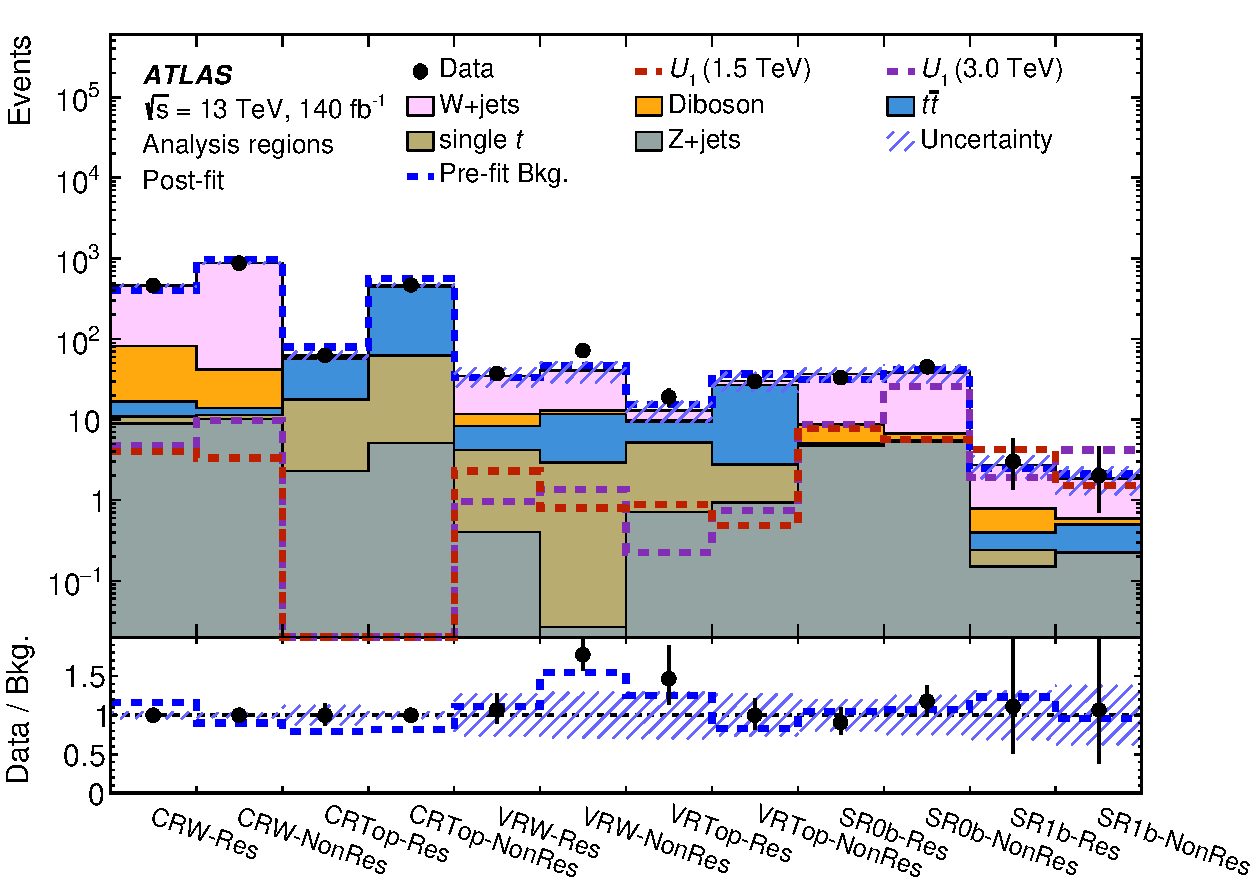
\includegraphics[width=0.64\linewidth]{Figs/CH10/yield_summary.pdf}
  \caption[Post-fit event yields in the CRs, VRs and SRs]{Comparison of the data and predicted background event yields for four CRs, four VRs and four SRs in the upper panel. The background prediction is shown after a background-only fit in the CRs. The signal expectation for $\mu=1$ is shown for illustrative purposes at the parameter points $(\MU,\gU,\beta_L^{23})=(1.5~\TeV,1.5,0.6)$ and $(3.0~\TeV,2.5,1.0)$ with a red dashed line and a violet dashed line, respectively. The ratio of the data to the background prediction is shown in the lower panel, separately for post-fit (black points) and pre-fit (dashed blue line) background. The size of the combined statistical and systematic uncertainty in the background prediction is indicated by a blue hatched band.}
  \label{fig:ch10_yield_summary}
\end{figure}

\begin{figure}[htpb]
  \centering
  \begin{subfigure}{0.44\linewidth}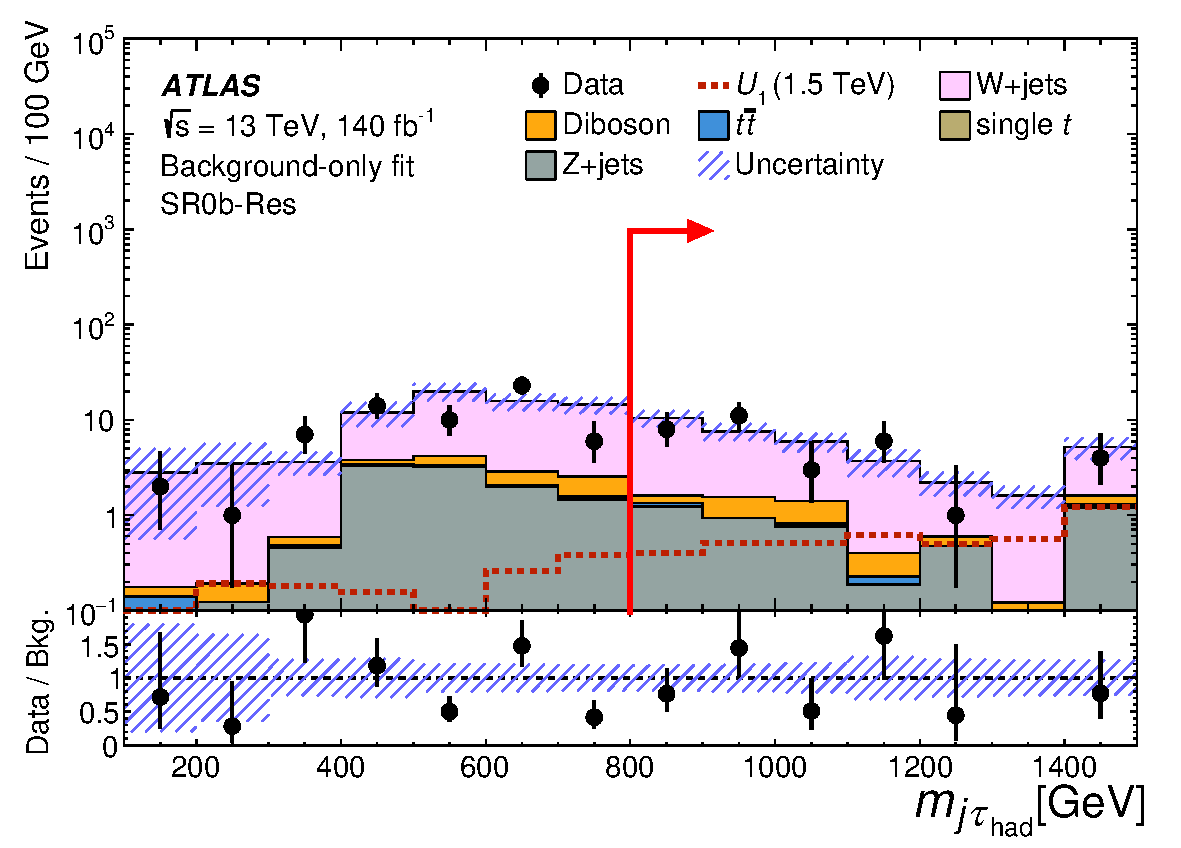
\includegraphics[width=\linewidth]{Figs/CH10/SR0b_Res_InvM.pdf}\caption{}\end{subfigure}\hfill
  \begin{subfigure}{0.44\linewidth}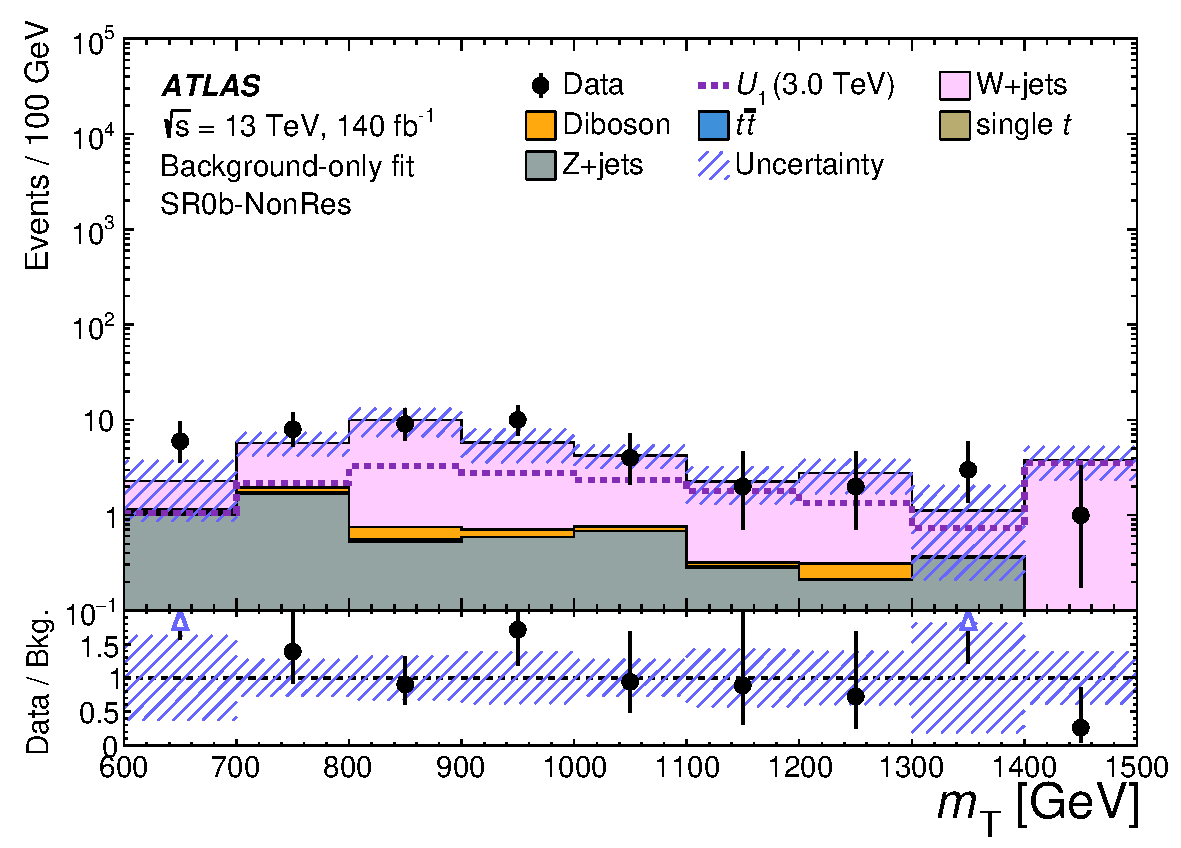
\includegraphics[width=\linewidth]{Figs/CH10/SR0b_NonRes_mT.pdf}\caption{}\end{subfigure}\\
  \begin{subfigure}{0.44\linewidth}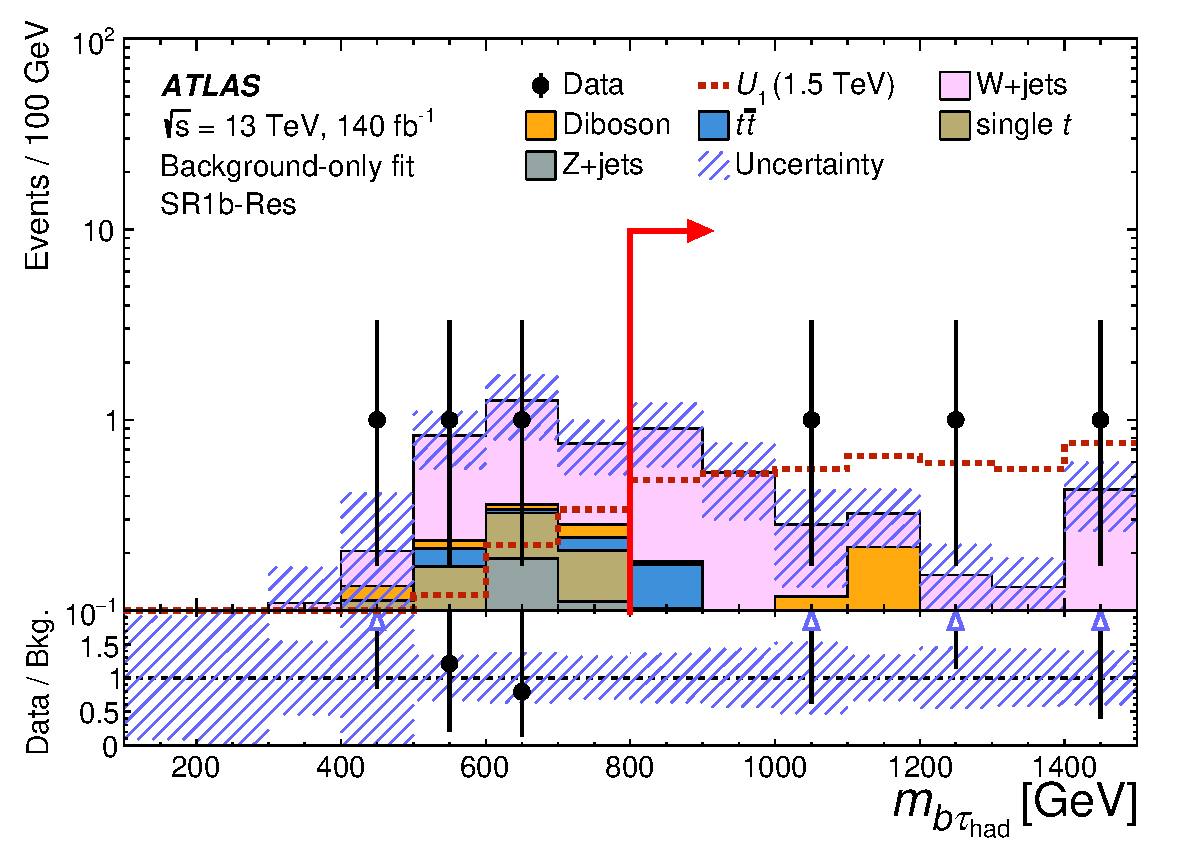
\includegraphics[width=\linewidth]{Figs/CH10/SR1b_Res_InvM.pdf}\caption{}\end{subfigure}\hfill
  \begin{subfigure}{0.44\linewidth}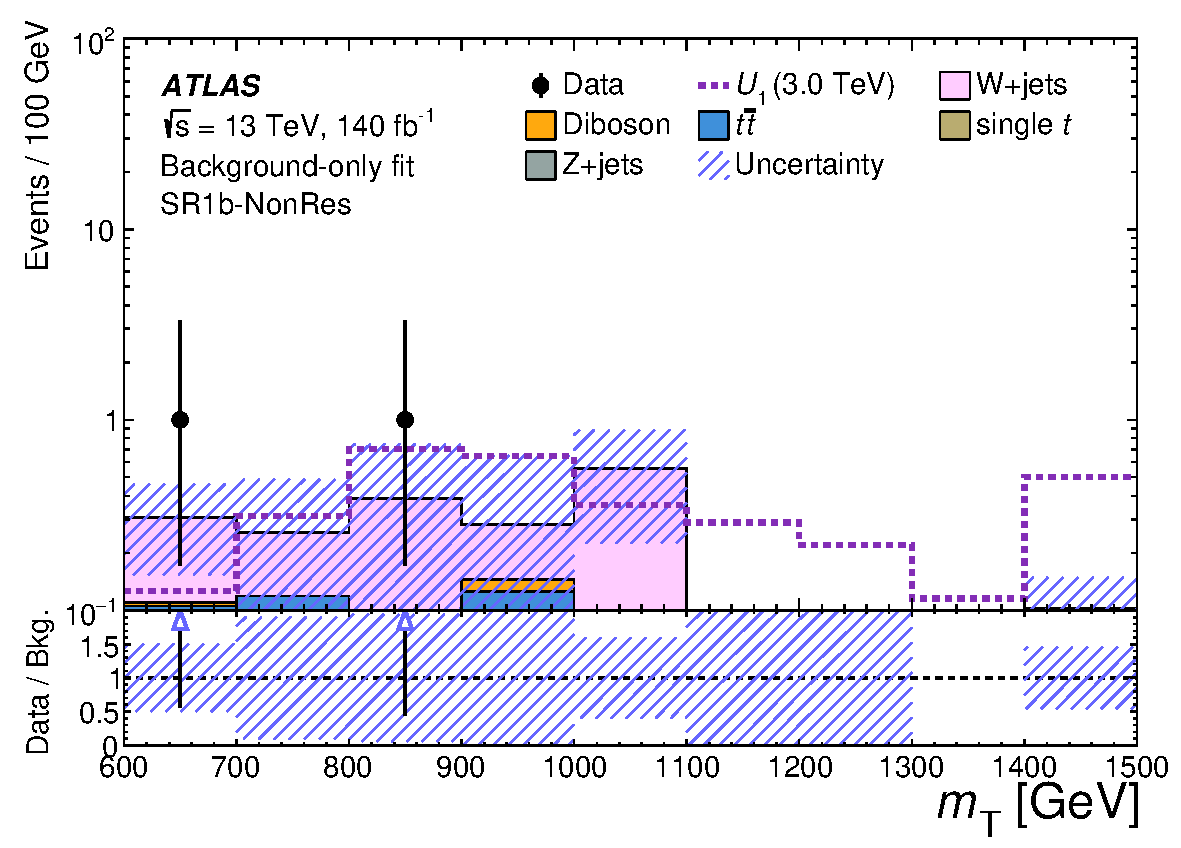
\includegraphics[width=\linewidth]{Figs/CH10/SR1b_NonRes_mT.pdf}\caption{}\end{subfigure}
  \caption[Unblinded mass and transverse-mass distributions]{N-1 distributions of (a) $m_{j\hadtau}$ in $\bVetoSR$-\Res, (b) $\mT$ in $\bVetoSR$-\NonRes, (c) $m_{b\hadtau}$ in $\bTagSR$-\Res and (d) $\mT$ in $\bTagSR$-\NonRes. The background-only fit is used for the background prediction. The signal expectations at parameter points $(\MU,\gU,\beta_L^{23})=(1.5~\TeV,1.5,0.6)$ and $(3.0~\TeV,2.5,1.0)$ are shown as red dashed lines in (a) and (c) and violet dashed lines in (b) and (d), respectively. The hatched bands show the combined statistical and systematic uncertainties. The bottom panels show the ratio of data to background prediction. Blue upward triangles indicate ratio values exceeding the displayed range. Red arrows indicate variable thresholds for the SRs. The last bin includes overflow.}
  \label{fig:ch10_sr_mass}
\end{figure}
 
\begin{figure}[htpb]
   \centering
   \begin{subfigure}{0.44\linewidth}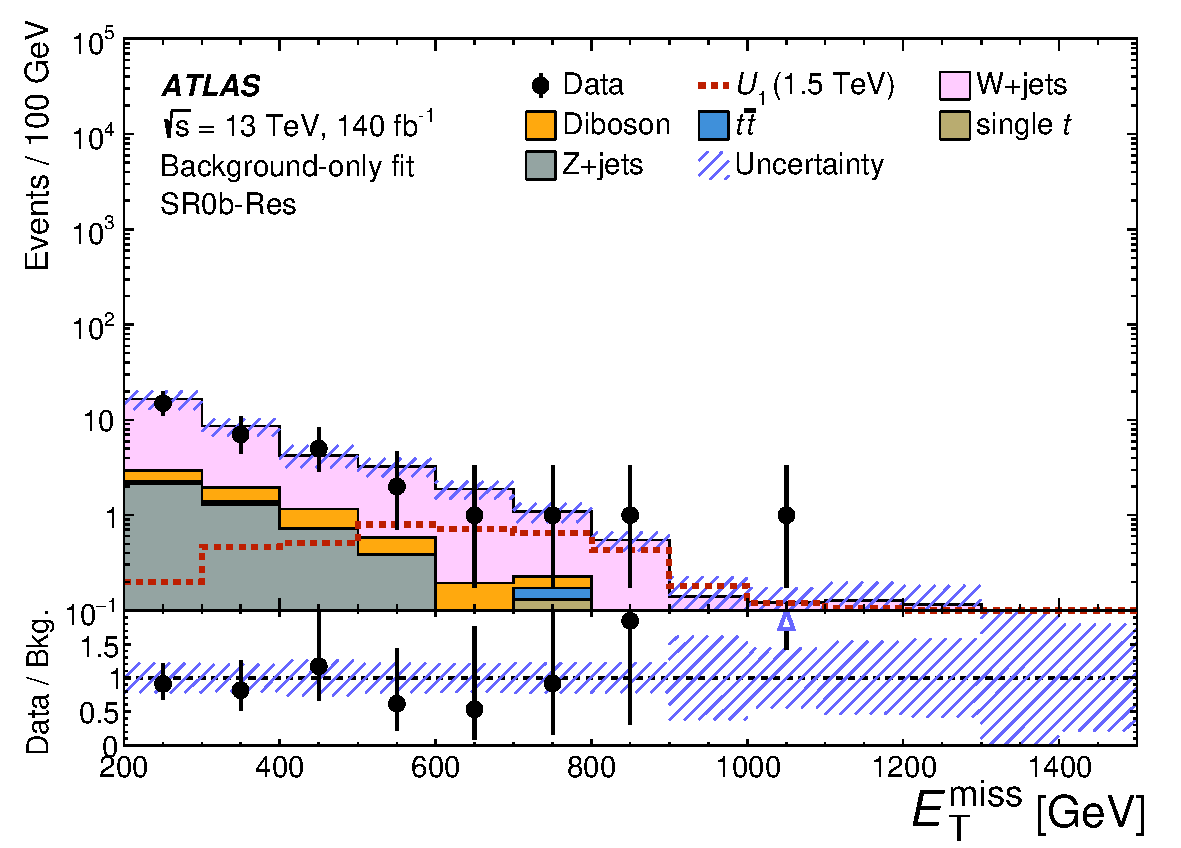
\includegraphics[width=\linewidth]{Figs/CH10/SR0b_Res_met.pdf}\caption{}\end{subfigure}\hfill
   \begin{subfigure}{0.44\linewidth}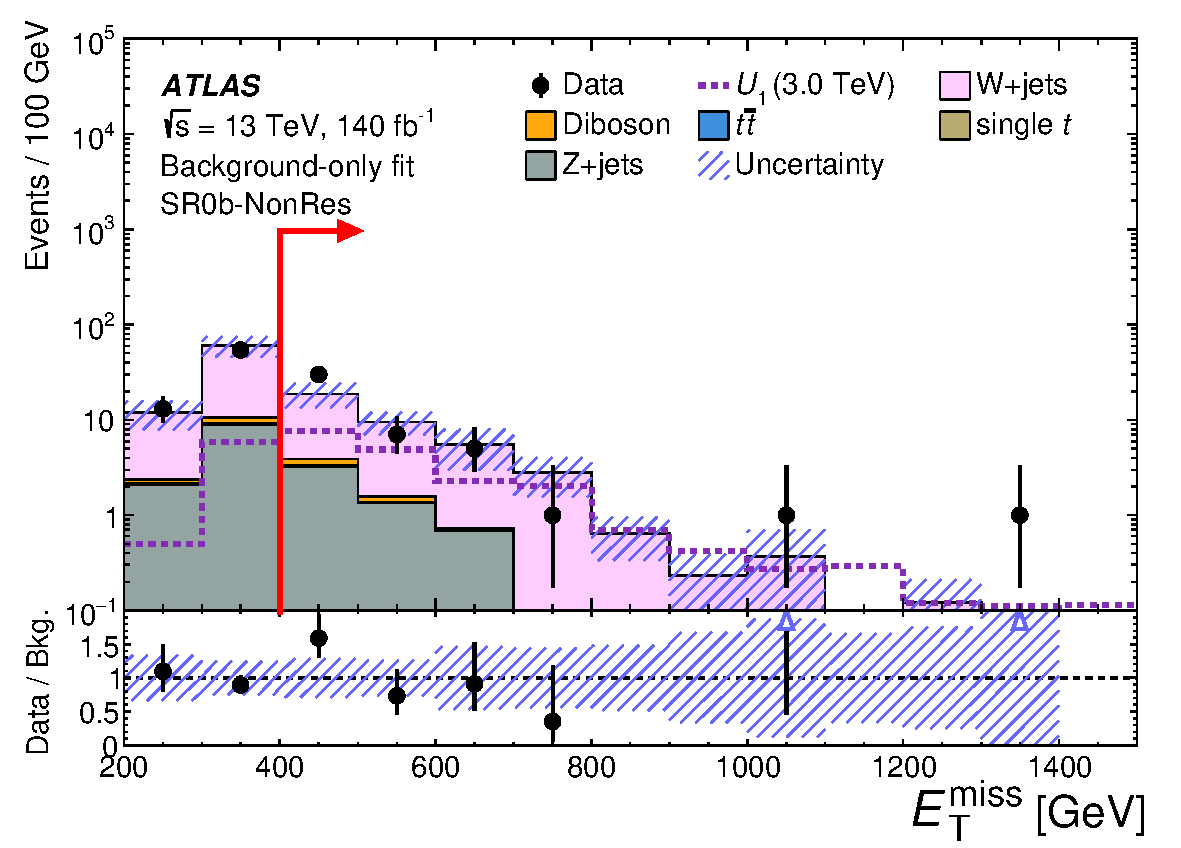
\includegraphics[width=\linewidth]{Figs/CH10/SR0b_NonRes_met.pdf}\caption{}\end{subfigure}\\
   \begin{subfigure}{0.44\linewidth}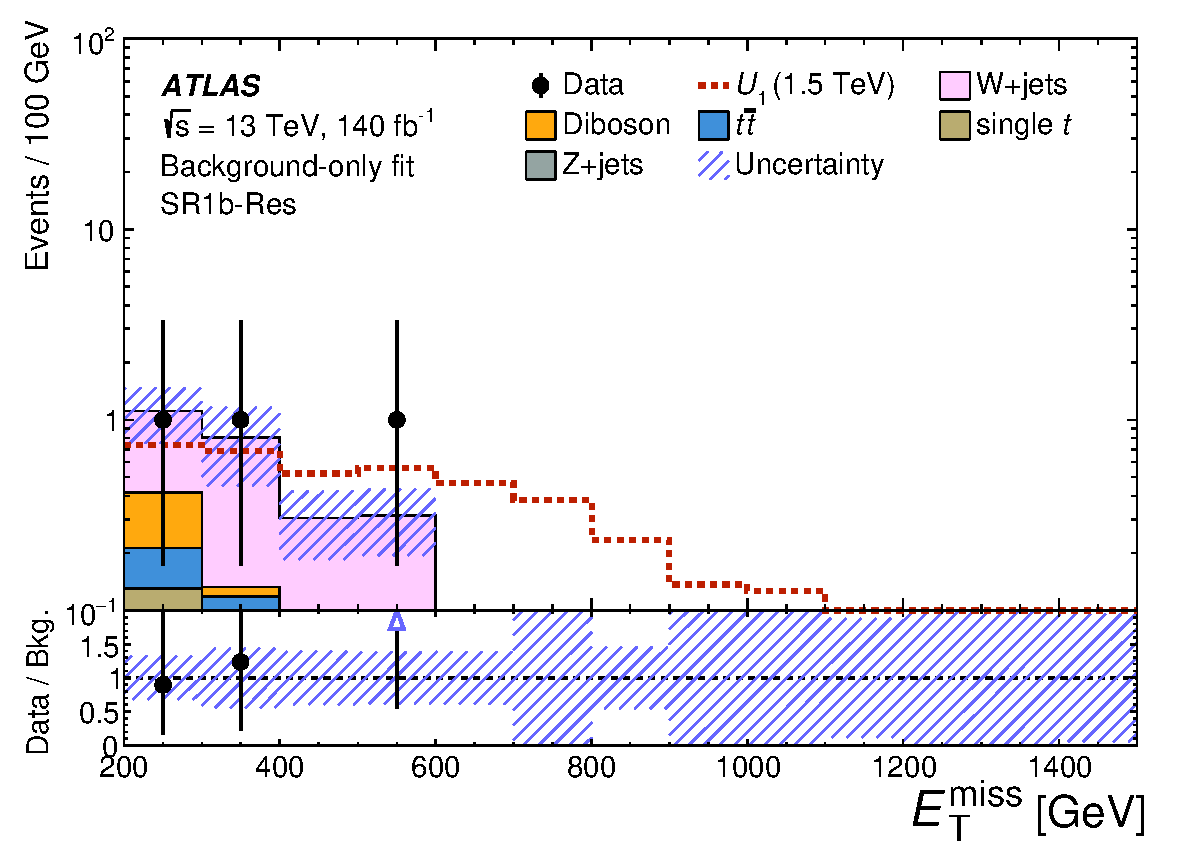
\includegraphics[width=\linewidth]{Figs/CH10/SR1b_Res_met.pdf}\caption{}\end{subfigure}\hfill
   \begin{subfigure}{0.44\linewidth}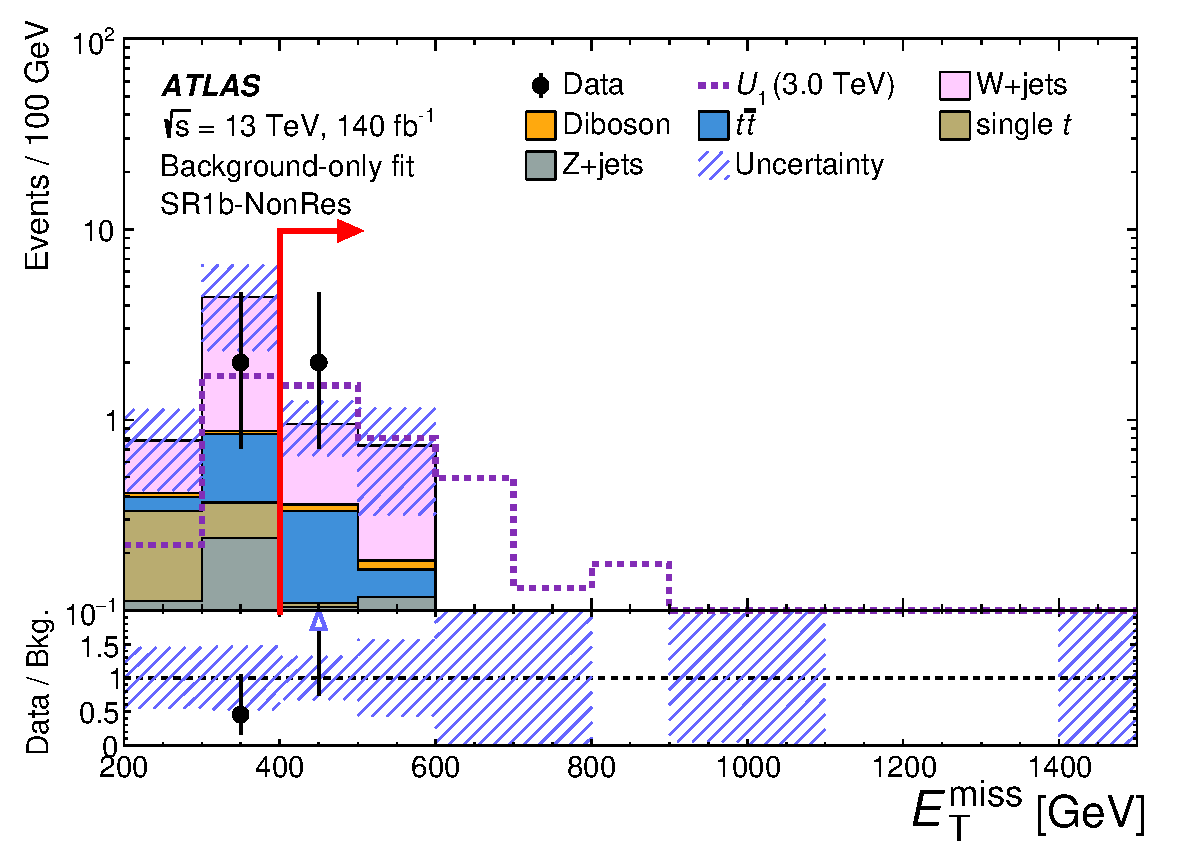
\includegraphics[width=\linewidth]{Figs/CH10/SR1b_NonRes_met.pdf}\caption{}\end{subfigure}
   \caption[Unblinded $\met$ distributions]{The unblinded N-1 $\met$ distributions in (a) $\bVetoSR$-\Res, (b) $\bVetoSR$-\NonRes, (c) $\bTagSR$-\Res and (d) $\bTagSR$-\NonRes before the $\met$ requirement. The background-only fit is used for the background prediction. The signal expectations at parameter points $(\MU,\gU,\beta_L^{23})=(1.5~\TeV,1.5,0.6)$ and $(3.0~\TeV,2.5,1.0)$ are shown as red dashed lines in (a) and (c) and violet dashed lines in (b) and (d), respectively. The hatched bands show the combined statistical and systematic uncertainties. The bottom panels show the ratio of data to background prediction. Blue upward triangles indicate ratio values exceeding the displayed range. Red arrows indicate variable thresholds for the SRs.}
   \label{fig:ch10_sr_met}
\end{figure} 

\clearpage
% Figure~\ref{fig:ch10_pulls} shows the NP pulls which are expressed by:
The NP pulls are defined as:
\begin{align}
 \mathrm{pull}=\frac{\hat\theta-\theta_{0}}{\Delta\theta},
 \label{eq:ch10_np_pull}
\end{align}
where $\theta_{0}$ and $\Delta\theta$ are the nominal NP value and pre-fit uncertainty, respectively.
The NP is considered to be constrained by the data if the normalised uncertainty is smaller than one.

The fit results show that the NPs remain close to their pre-fit values and their uncertainties are nearly unchanged.
This is expected, as differences between the observed and simulated yields in the CRs can mostly be absorbed by the free NFs.

% \begin{figure}[htpb]
%  \centering
%  \begin{minipage}[t]{0.48\linewidth}
%   \vspace{0pt}
%   \includegraphics[width=\linewidth]{Figs/CH10/pull_bonly_jet.pdf}
%  \end{minipage}\hfill
%  \begin{minipage}[t]{0.48\linewidth}
%   \vspace{0pt}
%   \includegraphics[width=\linewidth]{Figs/CH10/pull_bonly_theory.pdf}\\
%   \includegraphics[width=\linewidth]{Figs/CH10/pull_bonly_tau.pdf}\\
%   \includegraphics[width=\linewidth]{Figs/CH10/pull_bonly_muon.pdf}\\
%   \includegraphics[width=\linewidth]{Figs/CH10/pull_bonly_electron.pdf}\\
%   \includegraphics[width=\linewidth]{Figs/CH10/pull_bonly_other.pdf}
%  \end{minipage}
%  \caption[NP pulls in the CR fit]{NP pulls after the background-only fit in the CRs. Horizontal bars show the post-fit uncertainties. The green and yellow bands show the pre-fit $\pm1\sigma$ and $\pm2\sigma$ ranges, respectively.} \label{fig:ch10_pulls}
% \end{figure}

The correlations among the NPs are also studied.
These correlations are included through the post-fit covariance matrix when evaluating the uncertainties in the expected background yields.
In the S+B fit, they also affect the uncertainty on $\hat\mu$.
The leading correlations involve the TES detector NP and the top-quark NFs, while subleading correlations are observed between the muon momentum-resolution and trigger-efficiency NPs and the $\wjets$ NFs.
As shown in Fig.~\ref{fig:ch10_cr_np_variations}, pre-fit $\pm1\sigma$ variations of the TES detector NP change the top-quark background yield by $11.2\%$ and $17.4\%$ in $\CRTop$-\Res and $\CRTop$-\NonRes, respectively, while the corresponding variations of the two muon NPs change the $\wjets$ yields in $\CRW$ by a few percent.
An NP variation that increases a dominant background yield in a CR can be compensated by a decrease in its NF, resulting in these correlations. Their impacts on the $\mu$ fit in the S+B fit are discussed in the following section.

\begin{figure}[htpb]
 \centering
 \begin{subfigure}[t]{0.48\linewidth}
  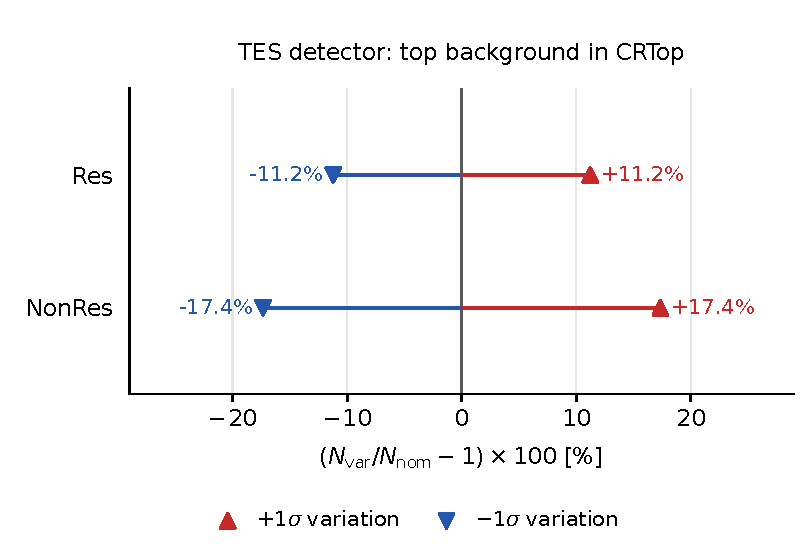
\includegraphics[width=\linewidth]{Figs/CH10/cr_np_yield_variations_top.pdf}
  \caption{}\label{fig:ch10_cr_np_variations_top}
 \end{subfigure}\hfill
 \begin{subfigure}[t]{0.48\linewidth}
  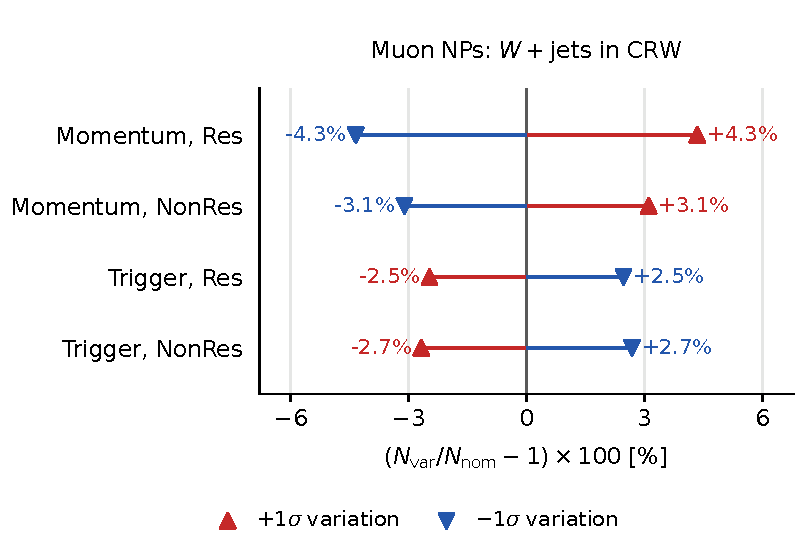
\includegraphics[width=\linewidth]{Figs/CH10/cr_np_yield_variations_muon.pdf}
  \caption{}\label{fig:ch10_cr_np_variations_muon}
 \end{subfigure}
 \caption[Effects of TES and muon NP variations on CR yields]{Changes of (a) the expected top-quark background ($\ttbar$ and single-top) yields in $\CRTop$ for TES detector variations and (b) the expected $\wjets$ yields in $\CRW$ for muon momentum-resolution and trigger-efficiency variations. Red and blue markers show the $+1\sigma$ and $-1\sigma$ variations, respectively.}
 \label{fig:ch10_cr_np_variations}
\end{figure}


\begin{table}[htbp]
 \caption[Post-fit yields in the CRs]{Observed and expected yields in the CRs after a background-only fit.}
 \label{tab:ch10_cr_yields}
 \centering\footnotesize
 \setstretch{1.0}
 \setlength{\tabcolsep}{3pt}
 \begin{tabular}{l|c|c|c|c}
 \toprule
 Process & \CRW-\Res & \CRW-\NonRes & \CRTop-\Res & \CRTop-\NonRes\\
 \midrule
 $\ttbar$ & $5.6\pm1.3$ & $2.6\pm0.6$ & $38.8\pm5.8$ & $385.5\pm19.1$\\
 Single-$t$ & $2.2\pm0.5$ & $1.1\pm0.2$ & $15.3\pm2.4$ & $57.9\pm3.8$\\
 $Z\to\ell\ell$+jets & $7.0\pm1.2$ & $9.5\pm1.2$ & $0.03\pm0.03$ & $0.42\pm0.44$\\
 $Z\to\nu\nu$+jets & $1.2\pm0.3$ & $0.42\pm0.16$ & $<0.01$ & $<0.01$\\
 $Z\to\tau\tau$+jets & $0.72\pm0.06$ & $0.28\pm0.08$ & $2.26\pm0.37$ & $4.73\pm0.60$\\
 $W$+jets & $380\pm22$ & $830\pm30$ & $3.0\pm0.7$ & $15.8\pm3.1$\\
 Diboson & $65.3\pm2.4$ & $28.0\pm1.9$ & $3.6\pm0.5$ & $3.7\pm0.5$\\
 \midrule
 Total & $462\pm22$ & $872\pm30$ & $63.0\pm7.9$ & $468\pm22$\\
 \midrule
 Data & 462 & 872 & 63 & 468\\
 \bottomrule
 \end{tabular}
\end{table}

\begin{table}[htbp]
 \caption[Post-fit yields in the VRs]{Observed and expected yields in the VRs after a background-only fit in the CRs.}
 \label{tab:ch10_vr_yields}
 \centering\footnotesize
 \setstretch{1.0}
 \setlength{\tabcolsep}{3pt}
 \begin{tabular}{l|c|c|c|c}
 \toprule
 Process & \VRW-\Res & \VRW-\NonRes & \VRTop-\Res & \VRTop-\NonRes\\
 \midrule
 $\ttbar$ & $4.1\pm1.8$ & $8.7\pm3.3$ & $4.18\pm1.76$ & $24.0\pm7.3$\\
 Single-$t$ & $3.8\pm1.6$ & $2.9\pm1.1$ & $4.54\pm1.93$ & $1.8\pm0.6$\\
 $Z\to\ell\ell$+jets & $0.37\pm0.16$ & $<0.01$ & $<0.01$ & $<0.01$\\
 $Z\to\nu\nu$+jets & $0.016\pm0.003$ & $0.03\pm0.02$ & $0.27\pm0.27$ & $0.78\pm0.78$\\
 $Z\to\tau\tau$+jets & $0.019\pm0.016$ & $<0.01$ & $0.44\pm0.15$ & $0.15\pm0.06$\\
 $W$+jets & $23.1\pm8.4$ & $27.8\pm10.6$ & $3.22\pm1.21$ & $3.3\pm1.4$\\
 Diboson & $3.3\pm1.2$ & $1.18\pm0.40$ & $0.31\pm0.11$ & $0.06\pm0.04$\\
 \midrule
 Total & $34.7\pm9.3$ & $40.7\pm12.0$ & $13.0\pm3.9$ & $30.1\pm8.1$\\
 \midrule
 Data & 37 & 72 & 19 & 30\\
 \bottomrule
 \end{tabular}
\end{table}

\begin{table}[htbp]
 \caption[Post-fit yields in the SRs]{Observed and expected yields in the SRs after a background-only fit in the CRs.}
 \label{tab:ch10_sr_yields}
 \centering\footnotesize
 \setstretch{1.0}
 \setlength{\tabcolsep}{3pt}
 \begin{tabular}{l|c|c|c|c}
 \toprule
 Process & $\bVetoSR$-\Res & $\bVetoSR$-\NonRes & $\bTagSR$-\Res & $\bTagSR$-\NonRes\\
 \midrule
 $\ttbar$ & $0.24\pm0.11$ & $0.11\pm0.10$ & $0.16\pm0.12$ & $0.27\pm0.13$\\
 Single-$t$ & $0.05\pm0.02$ & $0.02\pm0.01$ & $0.09\pm0.11$ & $<0.01$\\
 $Z\to\ell\ell$+jets & $0.03\pm0.03$ & $<0.01$ & $<0.01$ & $<0.01$\\
 $Z\to\nu\nu$+jets & $2.8\pm2.8$ & $2.3\pm2.3$ & $0.04\pm0.05$ & $0.05\pm0.06$\\
 $Z\to\tau\tau$+jets & $1.90\pm0.66$ & $3.1\pm1.2$ & $0.11\pm0.05$ & $0.17\pm0.06$\\
 $W$+jets & $27.7\pm6.0$ & $31.5\pm8.7$ & $1.9\pm0.7$ & $1.3\pm0.6$\\
 Diboson & $3.7\pm1.2$ & $1.18\pm0.47$ & $0.39\pm0.18$ & $0.10\pm0.04$\\
 \midrule
 Total & $36.4\pm7.3$ & $38.3\pm9.9$ & $2.69\pm0.83$ & $1.88\pm0.71$\\
 \midrule
 Data & 33 & 45 & 3 & 2\\
 \bottomrule
 \end{tabular}
\end{table}

\clearpage
\subsection{Unblinded S+B fit}
\label{subsec:ch10_sbfit}
Given that no significant excess is observed in the four SRs, the S+B fits have been performed for various signal parameters to set upper limits.
% The best-fit $\mu$ values are:
% \begin{align}
%  \hat\mu=0.00^{+0.58}_{-0.00}
% \end{align}
% at $(\MU,\gU,\beta_L^{23})=(1.5~\TeV,1.5,0.6)$,
% \begin{align}
%  \hat\mu=0.00^{+0.28}_{-0.00}
% \end{align}
% at $(\MU,\gU,\beta_L^{23})=(2.0~\TeV,2.0,1.0)$,
% \begin{align}
%  \hat\mu=0.00^{+0.39}_{-0.00}
% \end{align}
% at $(\MU,\gU,\beta_L^{23})=(2.5~\TeV,2.5,1.0)$, and
% \begin{align}
%  \hat\mu=0.30^{+0.50}_{-0.30}
%  \label{eq:ch10_observed_mu}
% \end{align}
% at $(\MU,\gU,\beta_L^{23})=(3.0~\TeV,2.5,1.0)$.
% The quoted uncertainties are the total fit uncertainties. The first three best-fit values lie at the $\mu=0$ boundary.

Two sets of signal parameters are picked to study the NP impacts in different LQ mass regions.
Figures~\ref{fig:ch10_rank_np_impacts_MLQ_1p5} and~\ref{fig:ch10_rank_np_impacts_MLQ_3p0} show the leading NP impacts at $(\MU,\gU,\beta_L^{23})=(1.5~\TeV,1.5,0.2)$ and $(3.0~\TeV,2.0,1.0)$, respectively, together with the pulls and post-fit uncertainties.
The corresponding best-fit values are
\begin{align}
 \hat\mu=0.35^{+2.62}_{-0.35}
 =0.35^{+2.47}_{-0.29}\,\mathrm{(stat)}
       ^{+0.45}_{-0.34}\,\mathrm{(syst)}
\end{align}
at $(\MU,\gU,\beta_L^{23})=(1.5~\TeV,1.5,0.2)$, and
\begin{align}
 \hat\mu=0.66^{+1.28}_{-0.66}
 =0.66^{+0.30}_{-0.64}\,\mathrm{(stat)}
       ^{+1.21}_{-0.51}\,\mathrm{(syst)}
\end{align}
at $(\MU,\gU,\beta_L^{23})=(3.0~\TeV,2.0,1.0)$.

The data statistical uncertainty dominates for $\MU=1.5~\TeV$, while both statistical and systematic uncertainties are important for $\MU=3.0~\TeV$.
For $\MU=1.5~\TeV$, the largest NP impact comes from the $\wjets$ heavy flavour uncertainty described in Section~\ref{subsec:ch9_wjets}, followed by the $\wjets$ QCD-scale uncertainties.
For $\MU=3.0~\TeV$, the TES detector NP gives the largest impact, followed by the $\wjets$ QCD-scale uncertainties.
This is expected: since the CRs use $e$/$\mu$ in place of $\hadtau$, the tau-related uncertainties are not cancelled out and remain important. And the uncertainties from $\wjets$ also have the large impact since it's the dominant background in the SRs.

\begin{figure}[htpb]
 \centering
 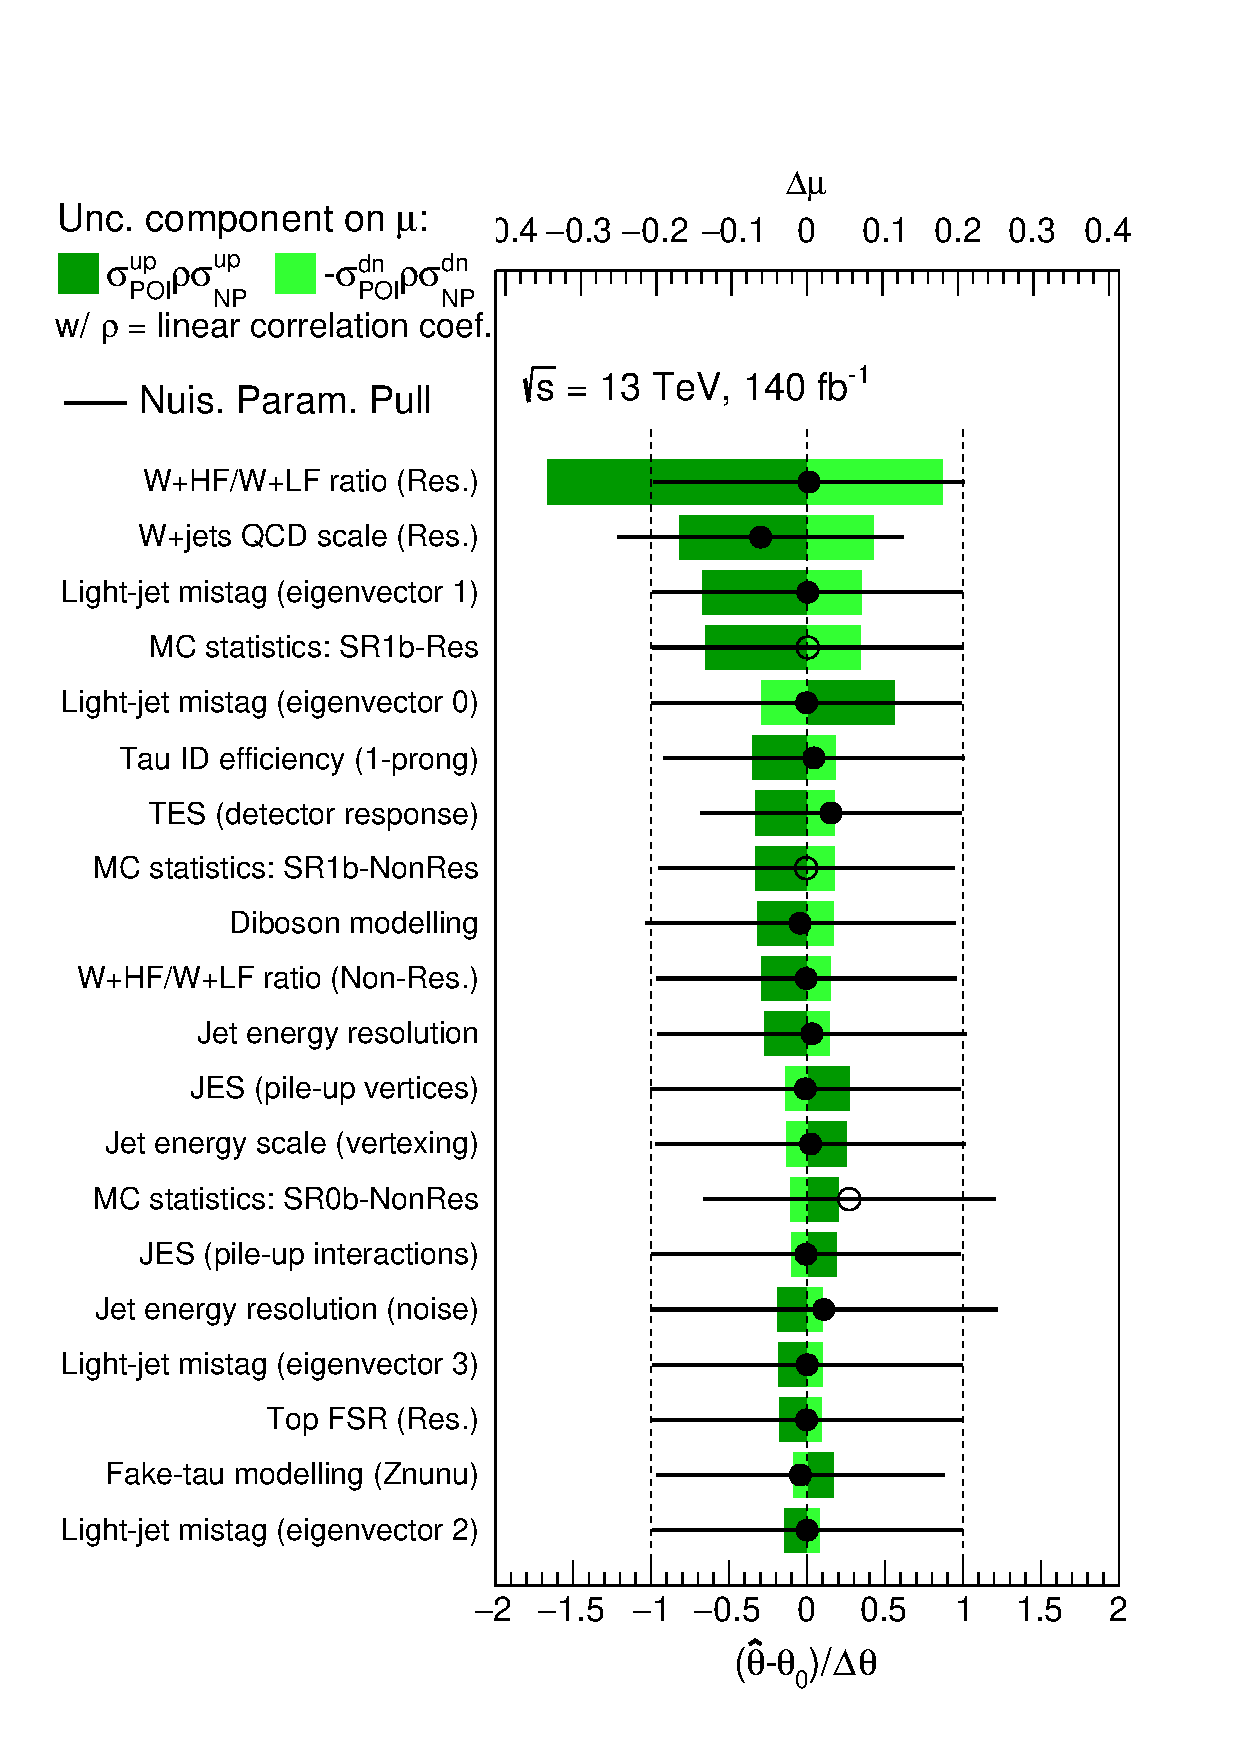
\includegraphics[width=0.95\linewidth]{Figs/CH10/rank_np_impacts_MLQ_1p5.pdf}
 \caption[Unblinded NP ranking for $\MU=1.5~\TeV$]{The unblinded ranking plot of NPs for $(\MU,\gU,\beta_L^{23})=(1.5~\TeV,1.5,0.2)$, using the four CRs and four SRs. NP impacts are obtained from the post-fit covariance matrix and are shown by the green bars. Black markers and horizontal error bars show the NP pulls and their post-fit uncertainties, respectively. The vertical dashed lines at $\pm1$ indicate the pre-fit $\pm1\sigma$ range. The quantity labelled $\Delta\mu$ represents the individual NP impacts on the fitted parameter $\sqrt{\mu}$. Most experimental systematic variations are symmetrised.}
 \label{fig:ch10_rank_np_impacts_MLQ_1p5}
\end{figure}

\begin{figure}[htpb]
 \centering
 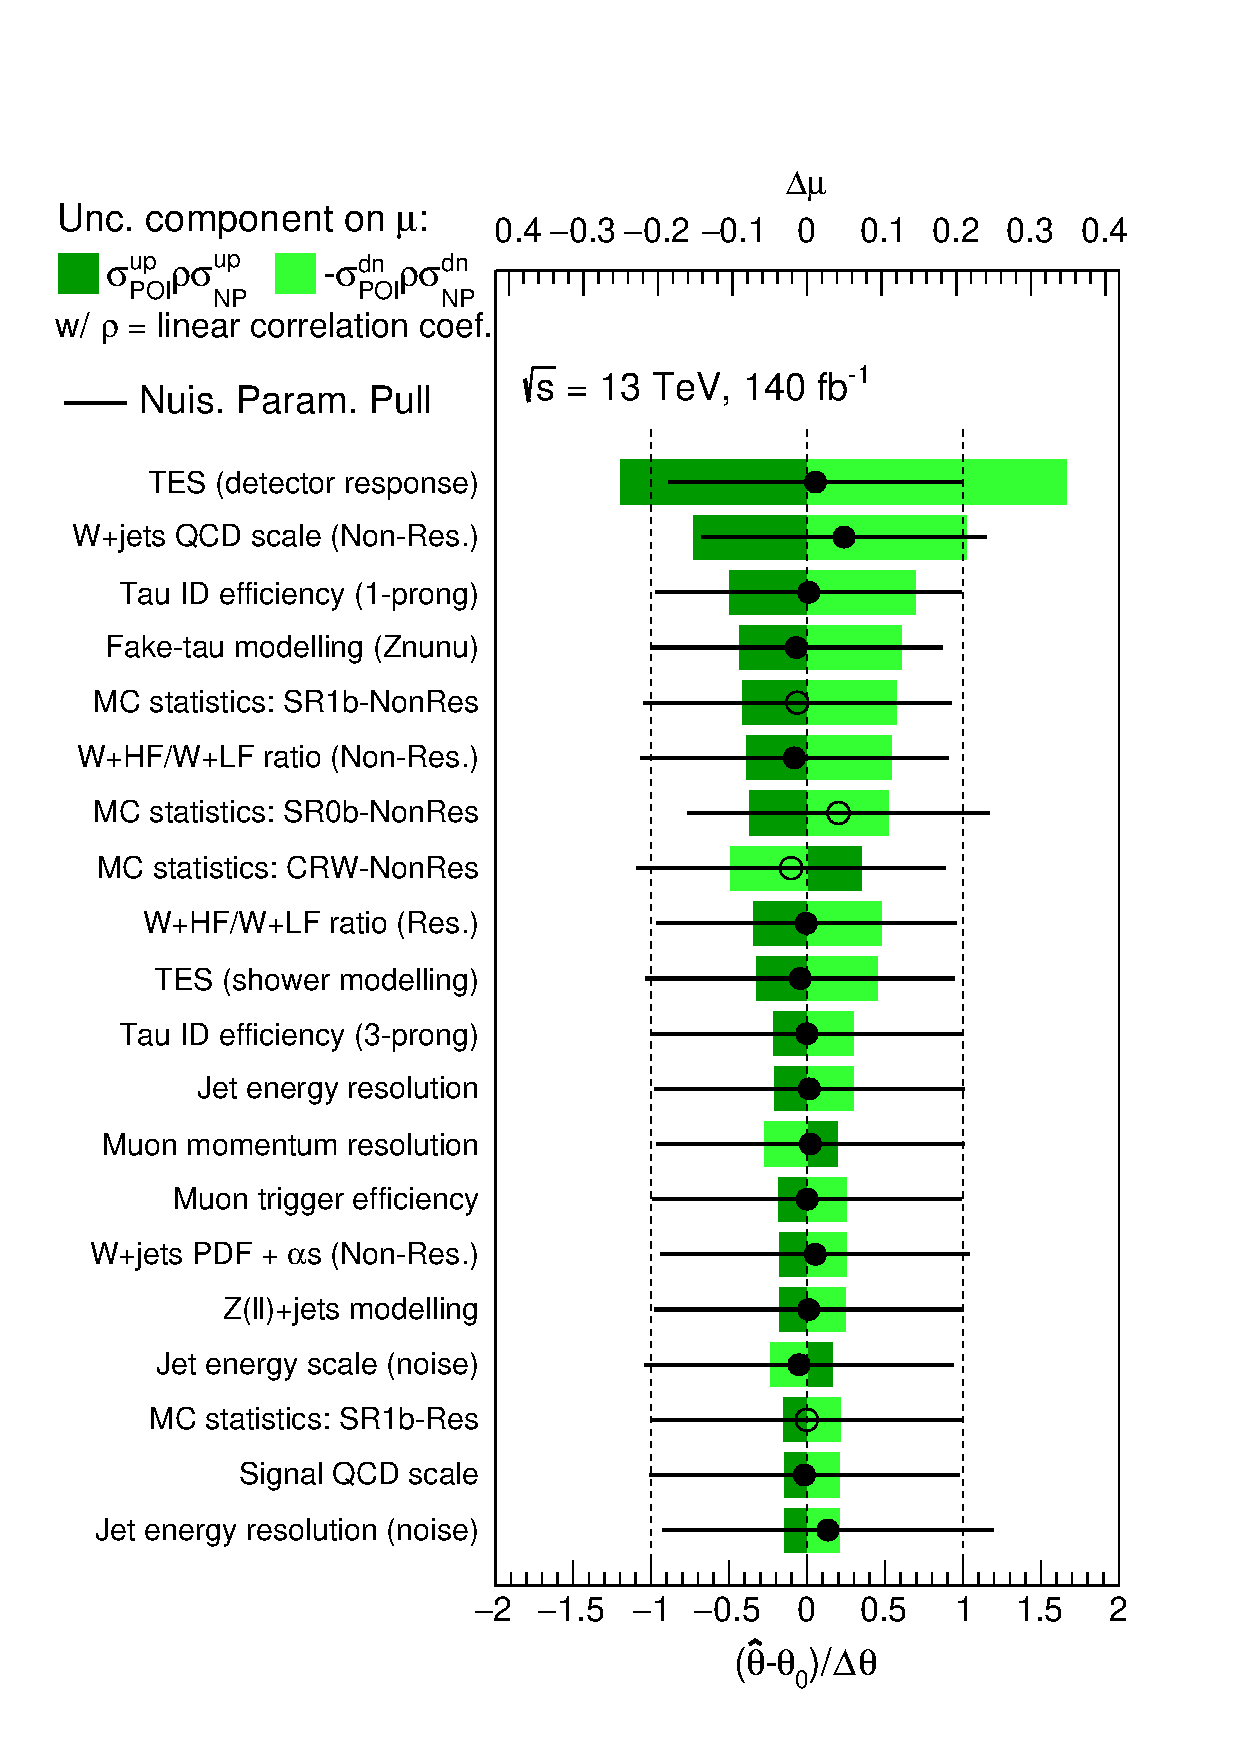
\includegraphics[width=0.95\linewidth]{Figs/CH10/rank_np_impacts_MLQ_3p0.pdf}
 \caption[Unblinded NP ranking for $\MU=3.0~\TeV$]{The unblinded ranking plot of NPs for $(\MU,\gU,\beta_L^{23})=(3.0~\TeV,2.0,1.0)$, using the four CRs and four SRs. NP impacts are obtained from the post-fit covariance matrix and are shown by the green bars. Black markers and horizontal error bars show the NP pulls and their post-fit uncertainties, respectively. The vertical dashed lines at $\pm1$ indicate the pre-fit $\pm1\sigma$ range. The quantity labelled $\Delta\mu$ represents the individual NP impacts on the fitted parameter $\sqrt{\mu}$. Most experimental systematic variations are symmetrised.}
 \label{fig:ch10_rank_np_impacts_MLQ_3p0}
\end{figure}

\clearpage
\section{Exclusion limits}
\label{sec:ch10_limits}

\subsection{left-handed scenario}
\label{subsec:ch10_limits_lh}

The contributions of the individual SRs are shown in Fig.~\ref{fig:ch10_sr_comparison} using asymptotic calculations.
As shown in Fig.~\ref{fig:ch10_sr_comparison}(a), the resonant SRs provide the stronger sensitivity at low mass, while the non-resonant SRs become more sensitive as on-shell production is suppressed at higher mass.
Their combination gives the best expected limit.
Meanwhile, as shown in Fig.~\ref{fig:ch10_sr_comparison}(b), $\bTagSR$ provides most of the sensitivity, while adding $\bVetoSR$ improves the combined limit particularly towards large $\beta_L^{23}$ and small $\gU$.
This is expected since the larger signal contribution without a $b$ jet would be enhanced by the second-generation coupling.
These comparisons explain the role of each SR. The exclusion limits are then obtained with pseudo-experiments.

\begin{figure}[htpb]
 \centering
 \begin{subfigure}{0.48\linewidth}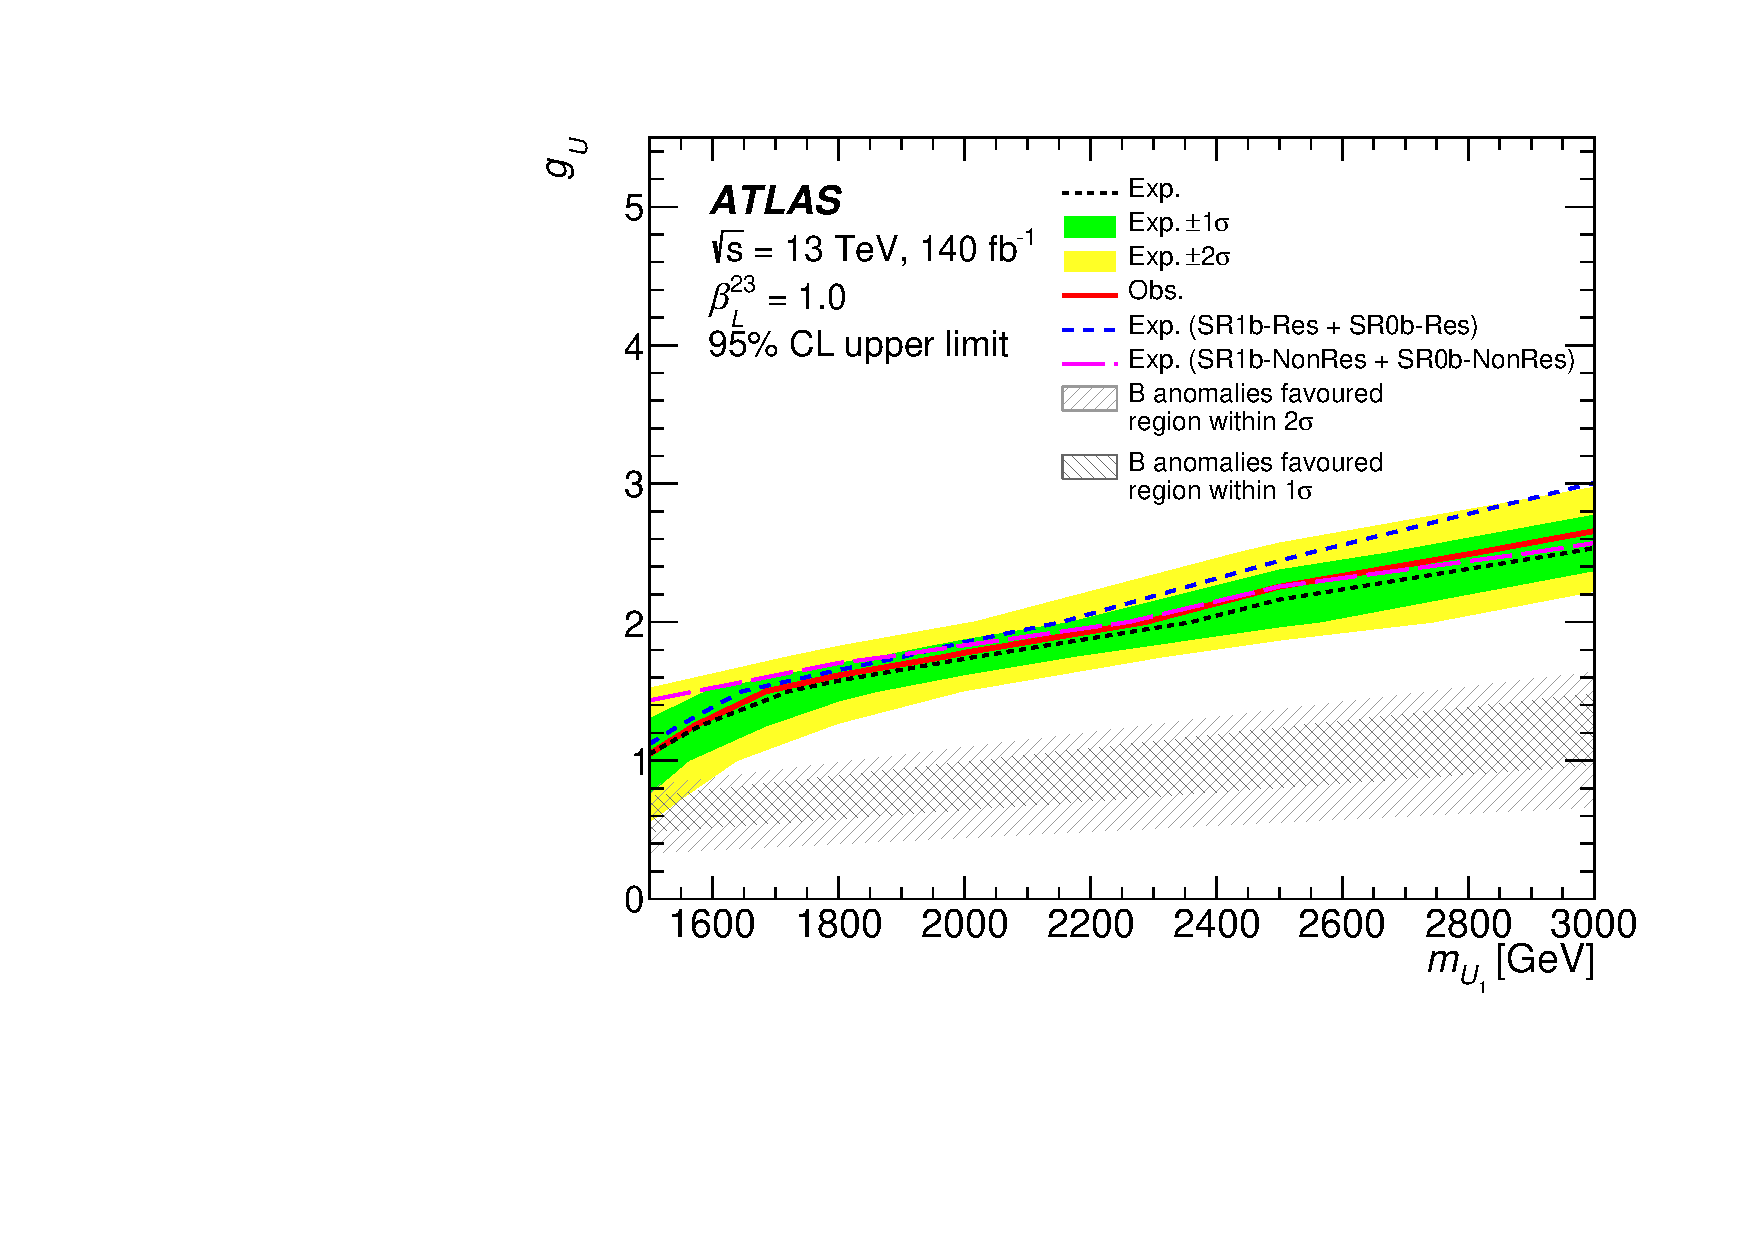
\includegraphics[width=\linewidth]{Figs/CH10/compare_res_nonres.pdf}\caption{}\end{subfigure}\hfill
 \begin{subfigure}{0.48\linewidth}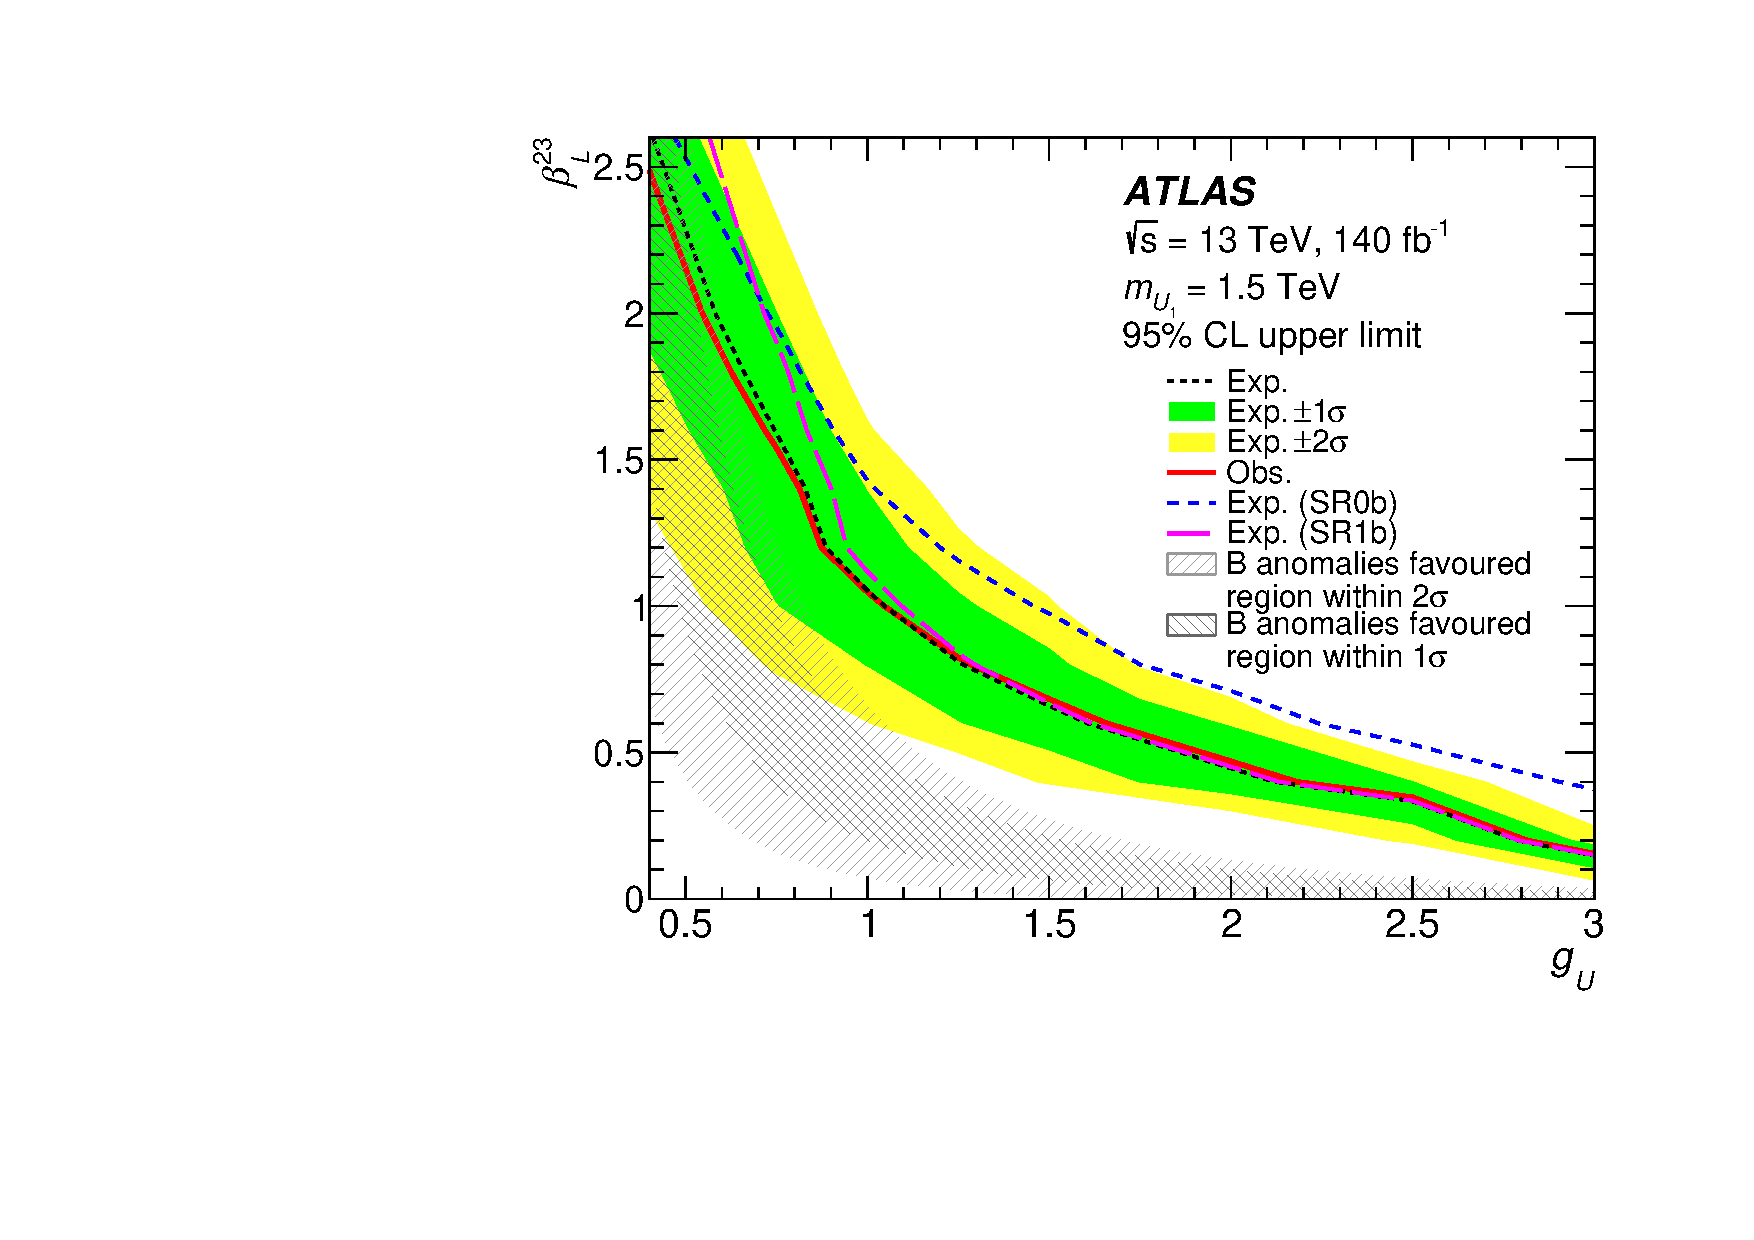
\includegraphics[width=\linewidth]{Figs/CH10/compare_sr0b_sr1b.pdf}\caption{}\end{subfigure}
 \caption[Contributions of the individual signal regions to the sensitivity]{Observed (red full line) and expected (black dashed line) 95\% CL upper limits on (a) $\gU$ as a function of $\MU$ at $\beta_L^{23}=1.0$ and (b) $\beta_L^{23}$ as a function of $\gU$ at $\MU=1.5~\TeV$. The shaded regions are favoured by $B$ anomalies at the $2\sigma$ level, converted from the $C_{LL}^{c}$ limit in Fig.~\ref{fig:cll_clr_low_energy_fit} using Eq.~\eqref{eq:cll_c_approx}. The individual expected limits from the resonant and non-resonant SRs are also overlaid in (a), and those from $\bVetoSR$ and $\bTagSR$ are overlaid in (b). In this figure, limits are calculated using the asymptotic formulae~\cite{Cowan:2010js} rather than pseudo-experiments.}
 \label{fig:ch10_sr_comparison}
\end{figure}

Figures~\ref{fig:ch10_limits_mass} and~\ref{fig:ch10_limits_couplings} present the 95\% CL exclusions for the purely left-handed scenario using all four SRs.
At $\MU=1.5~\TeV$, the observed (expected) upper limits on $\gU$ are 1.13 (1.11) for $\beta_L^{23}=1.0$ and 0.52 (0.53) for $\beta_L^{23}=2.2$.
At $\MU=2.5~\TeV$, they are 2.30 (2.19) and 1.22 (1.18), respectively.
The hatched regions are obtained by mapping the low-energy constraint on $C_{LL}^{c}$ shown in Fig.~\ref{fig:cll_clr_low_energy_fit} through Eq.~\eqref{eq:cll_c_approx}.
The results test the parameter space at large $\beta_L^{23}$ and complement the $b\tau$ searches discussed in Section~\ref{subsec:lq_searches_lhc}~\cite{ATLAS2023LQBTau}.

\begin{figure}[htpb]
 \centering
 \begin{subfigure}{0.47\linewidth}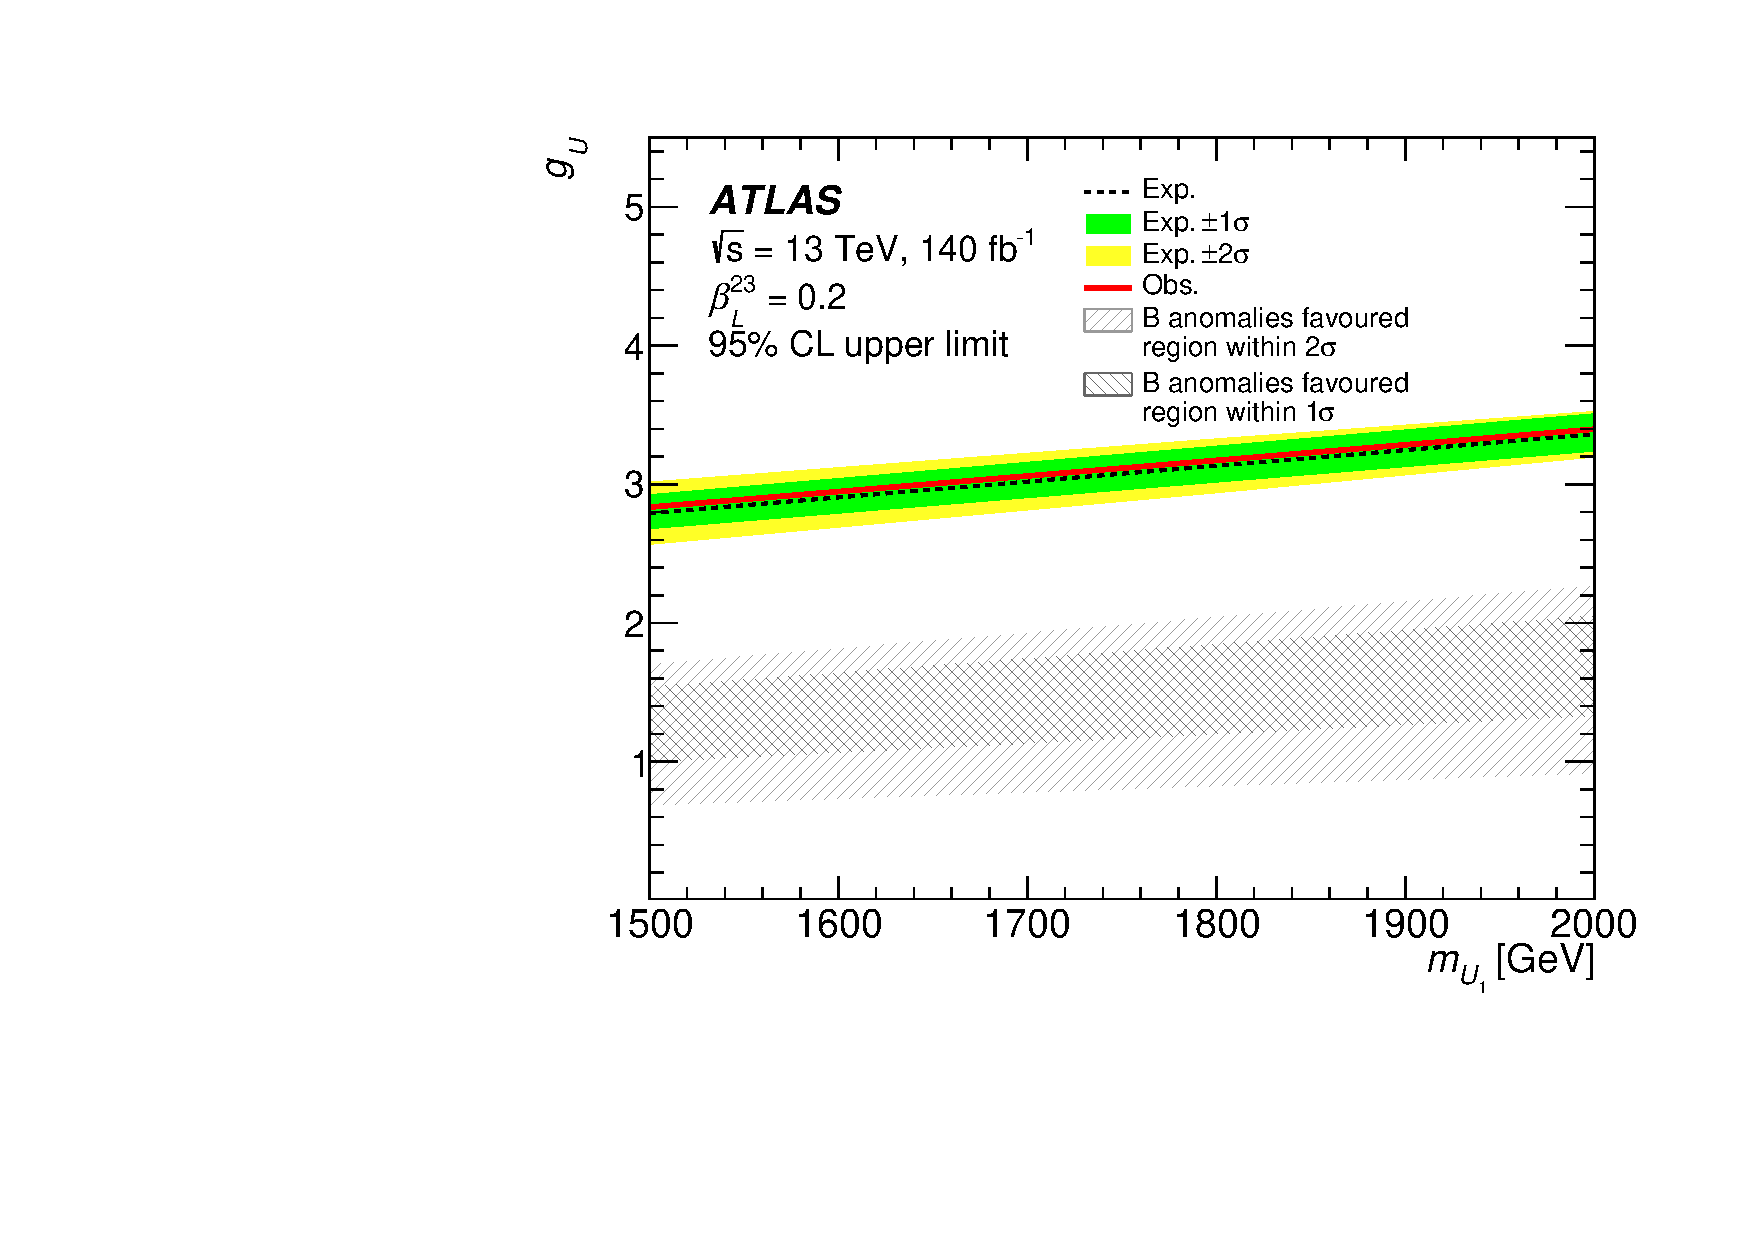
\includegraphics[width=\linewidth]{Figs/CH10/limit_beta0_2.pdf}\caption{}\end{subfigure}\\
 \begin{subfigure}{0.47\linewidth}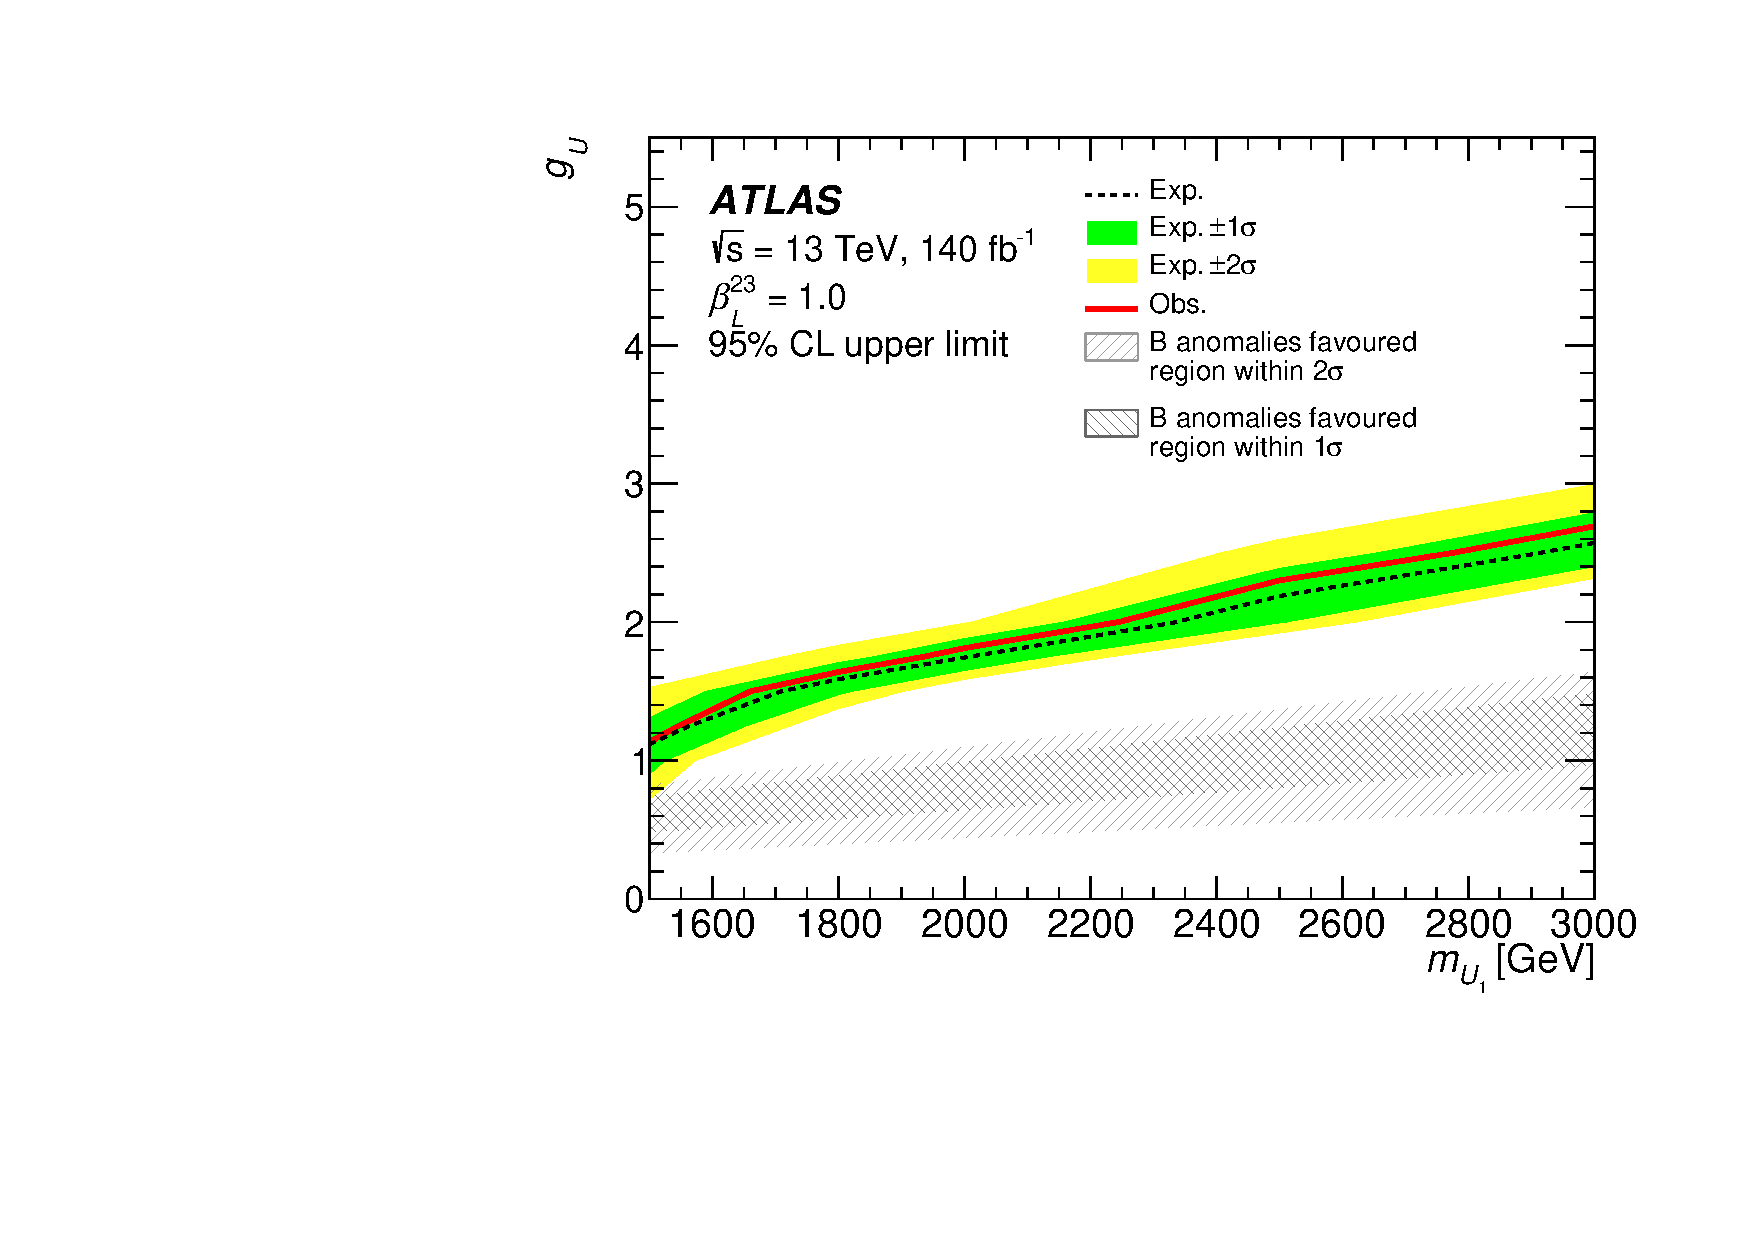
\includegraphics[width=\linewidth]{Figs/CH10/limit_beta1_0.pdf}\caption{}\end{subfigure}\hfill
 \begin{subfigure}{0.47\linewidth}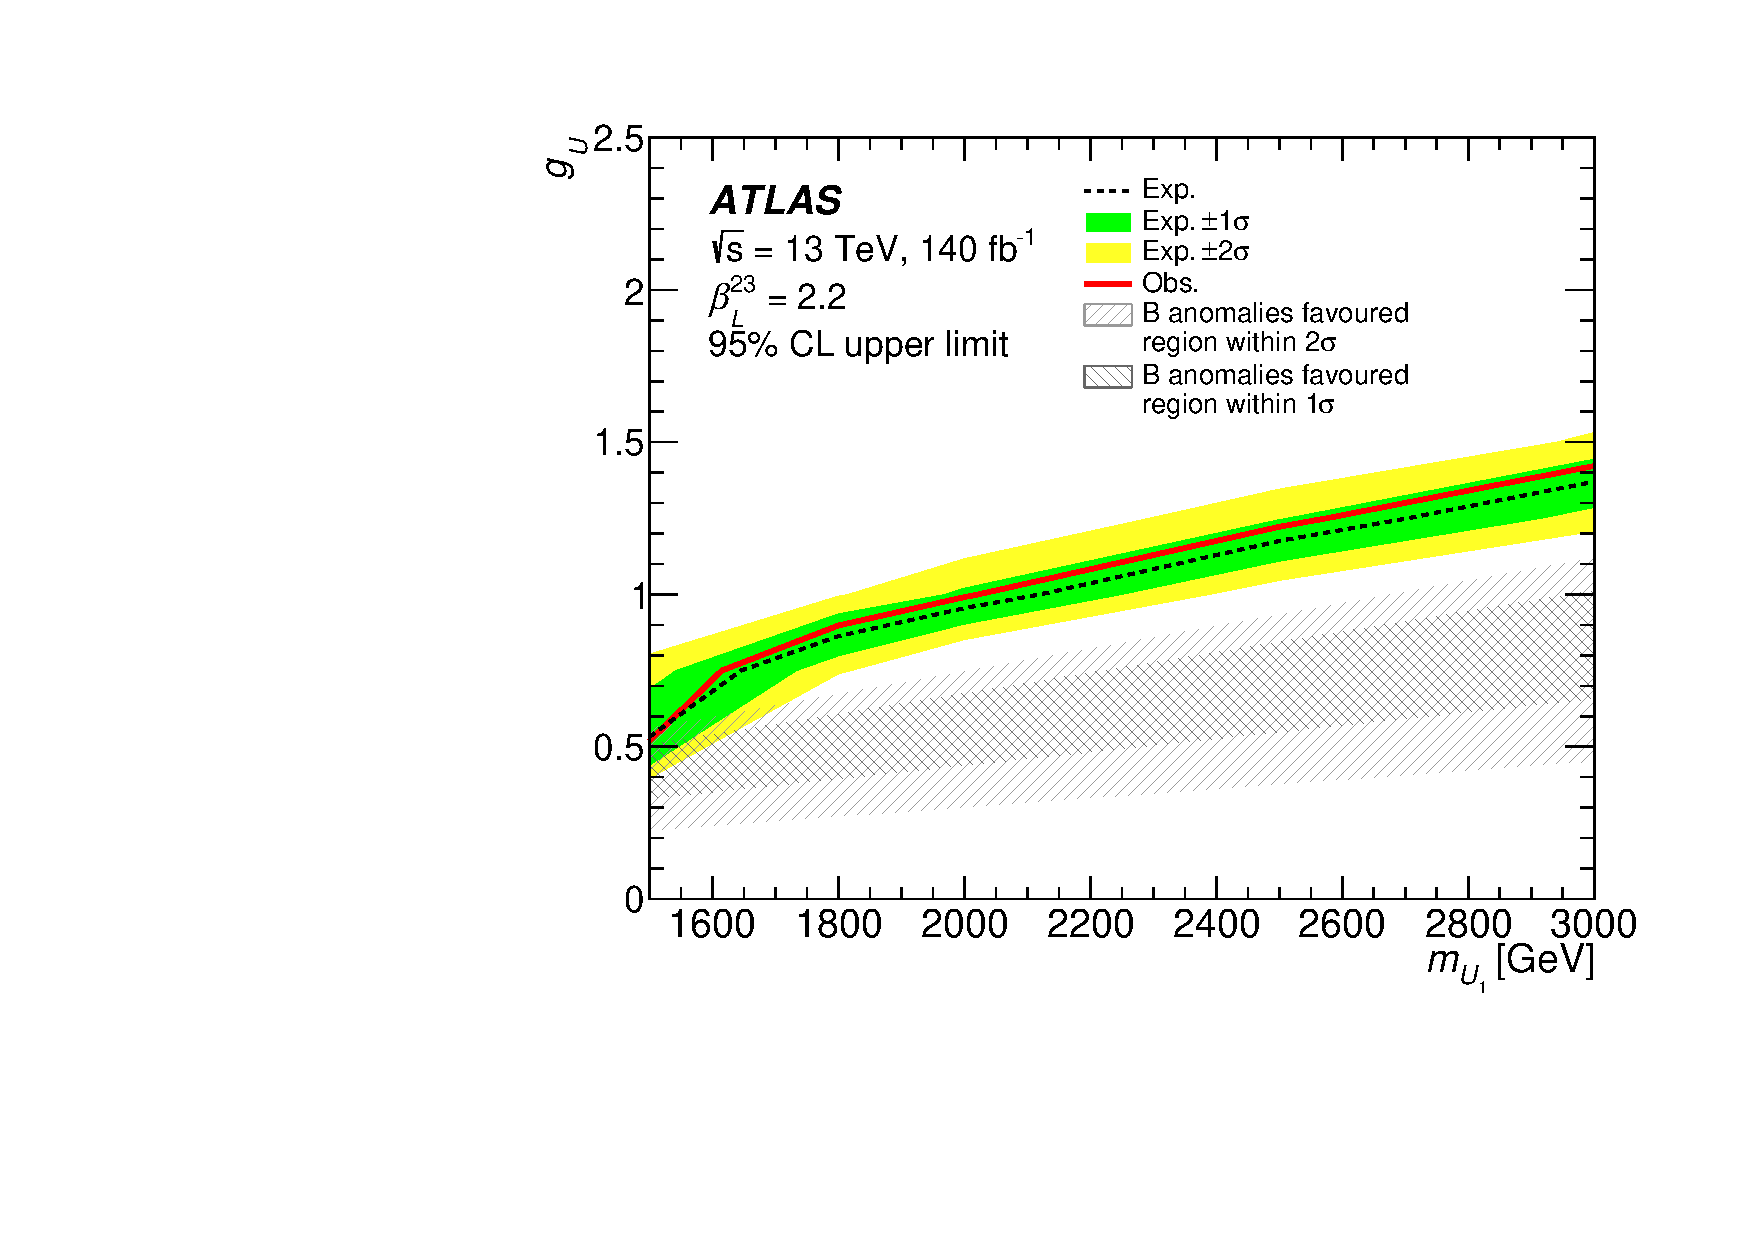
\includegraphics[width=\linewidth]{Figs/CH10/limit_beta2_2.pdf}\caption{}\end{subfigure}
 \caption[Limits on the coupling as a function of the leptoquark mass]{Observed (red full line) and expected (black dashed line) 95\% CL upper limits on $\gU$ as a function of $\MU$, at (a) $\beta_L^{23}=0.2$, (b) 1.0 and (c) 2.2. The shaded regions are favoured by $B$ anomalies at the $1\sigma$ and $2\sigma$ levels, converted from the $C_{LL}^{c}$ limit in Fig.~\ref{fig:cll_clr_low_energy_fit} using Eq.~\eqref{eq:cll_c_approx}.}
 \label{fig:ch10_limits_mass}
\end{figure}


\begin{figure}[htpb]
 \centering
 \begin{subfigure}{0.47\linewidth}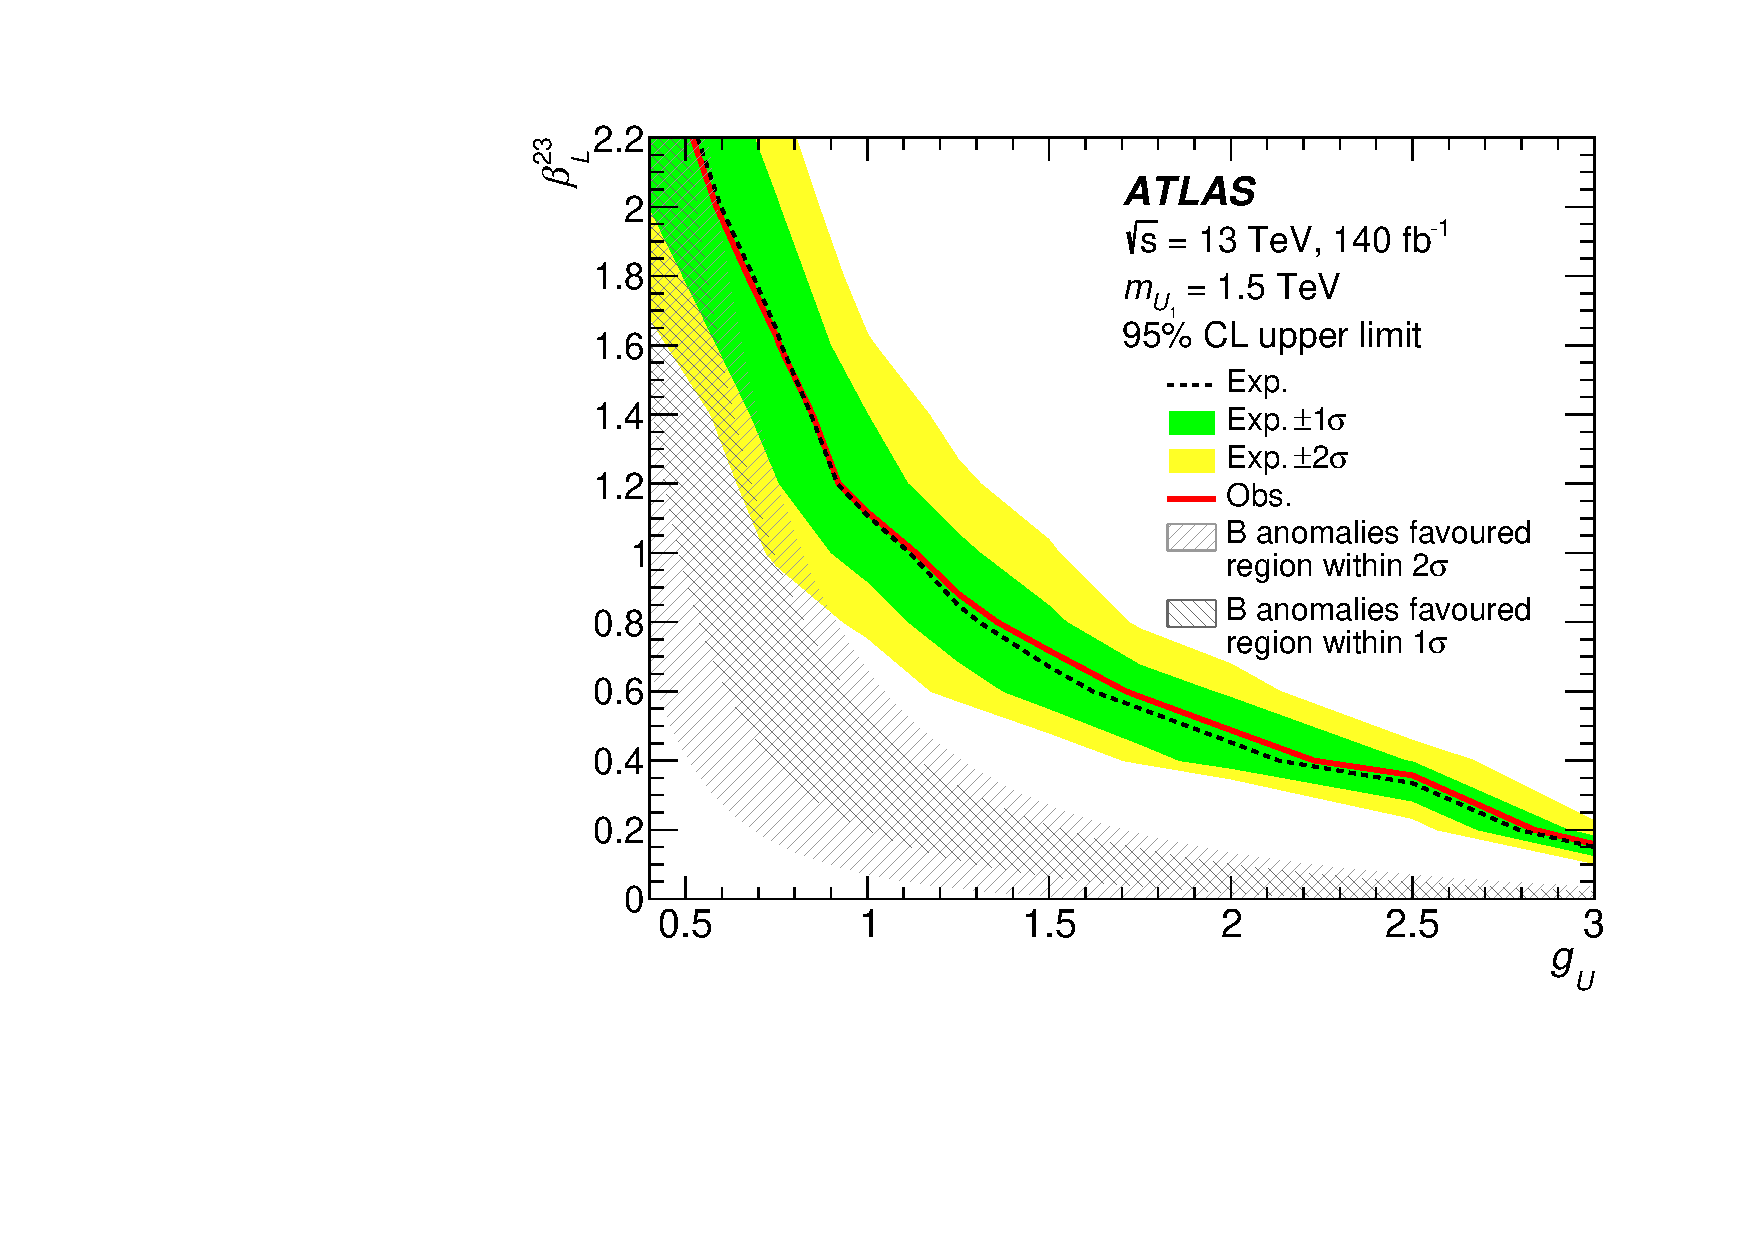
\includegraphics[width=\linewidth]{Figs/CH10/limit_mu1500.pdf}\caption{}\end{subfigure}\hfill
 \begin{subfigure}{0.47\linewidth}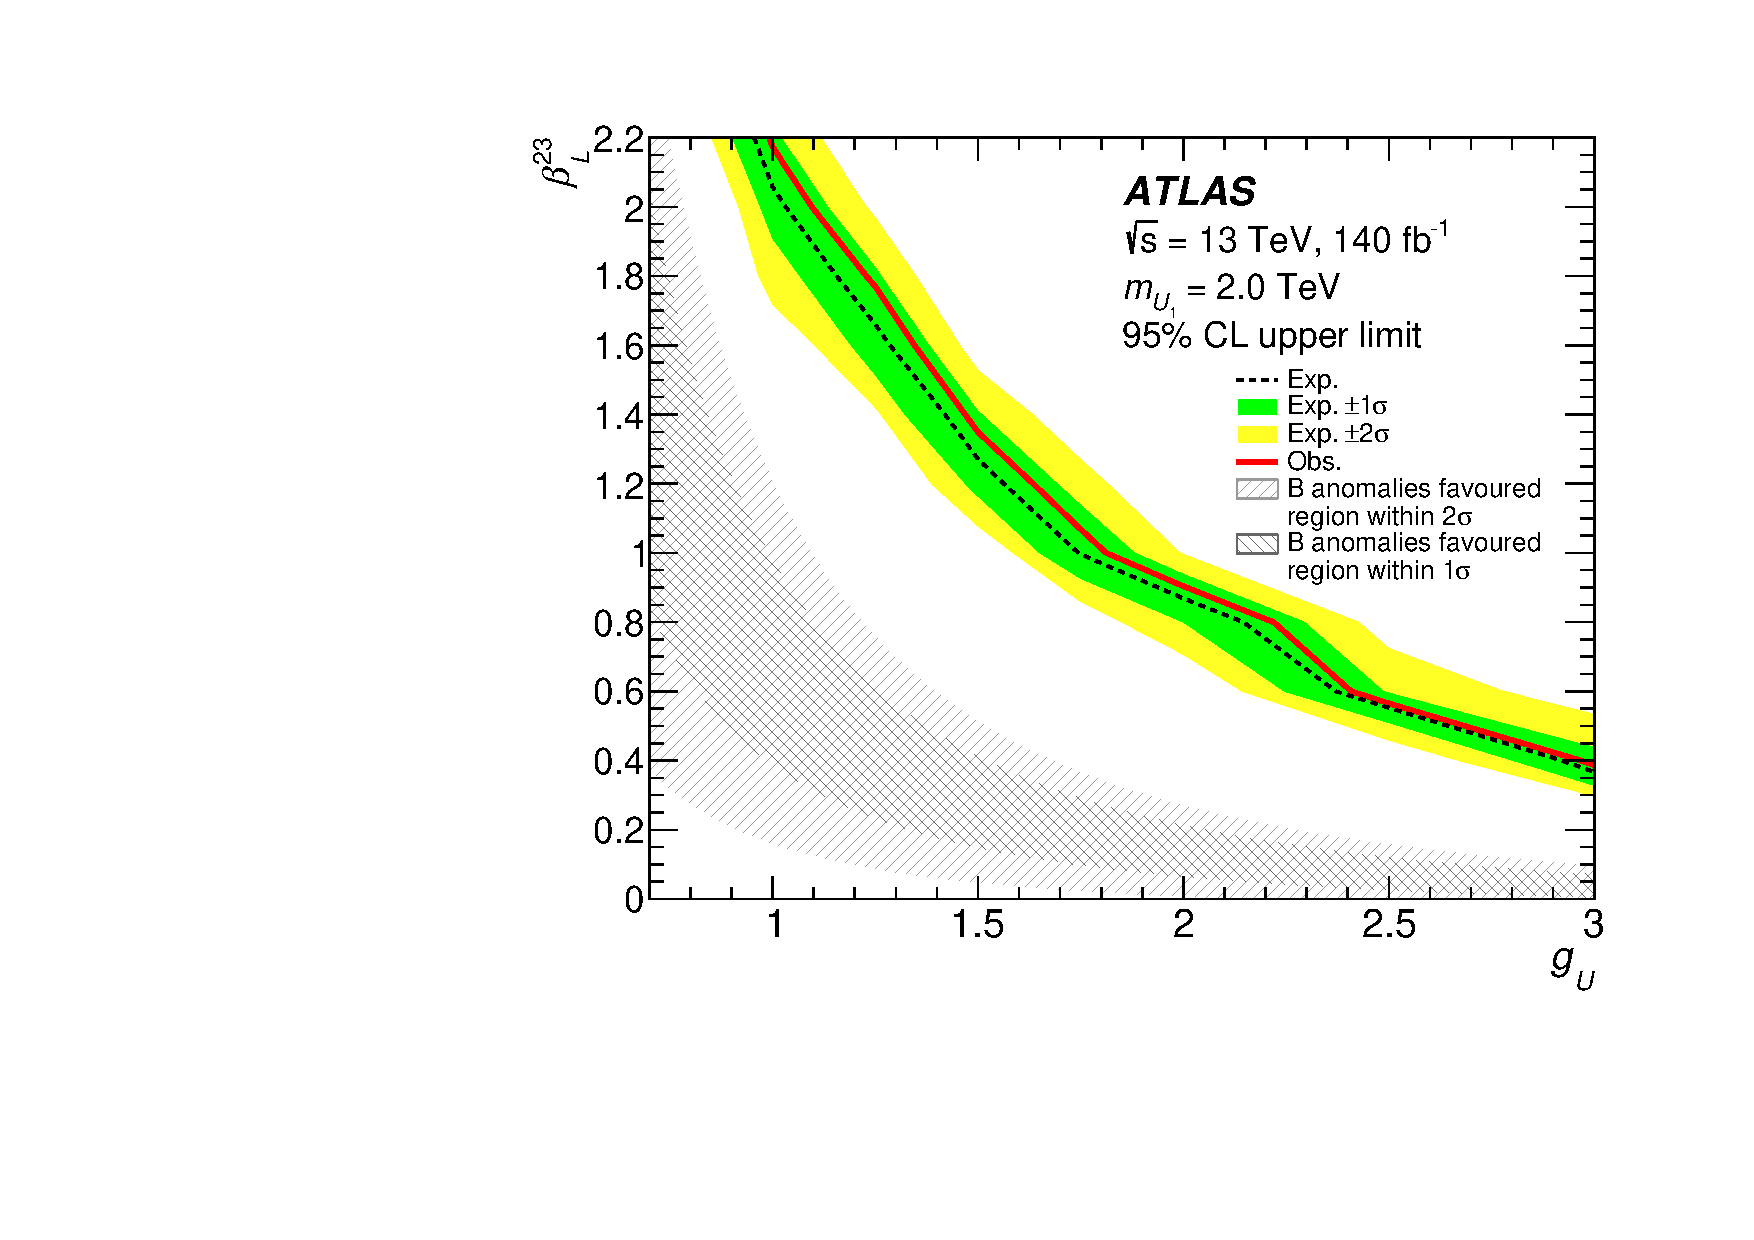
\includegraphics[width=\linewidth]{Figs/CH10/limit_mu2000.pdf}\caption{}\end{subfigure}\\
 \begin{subfigure}{0.47\linewidth}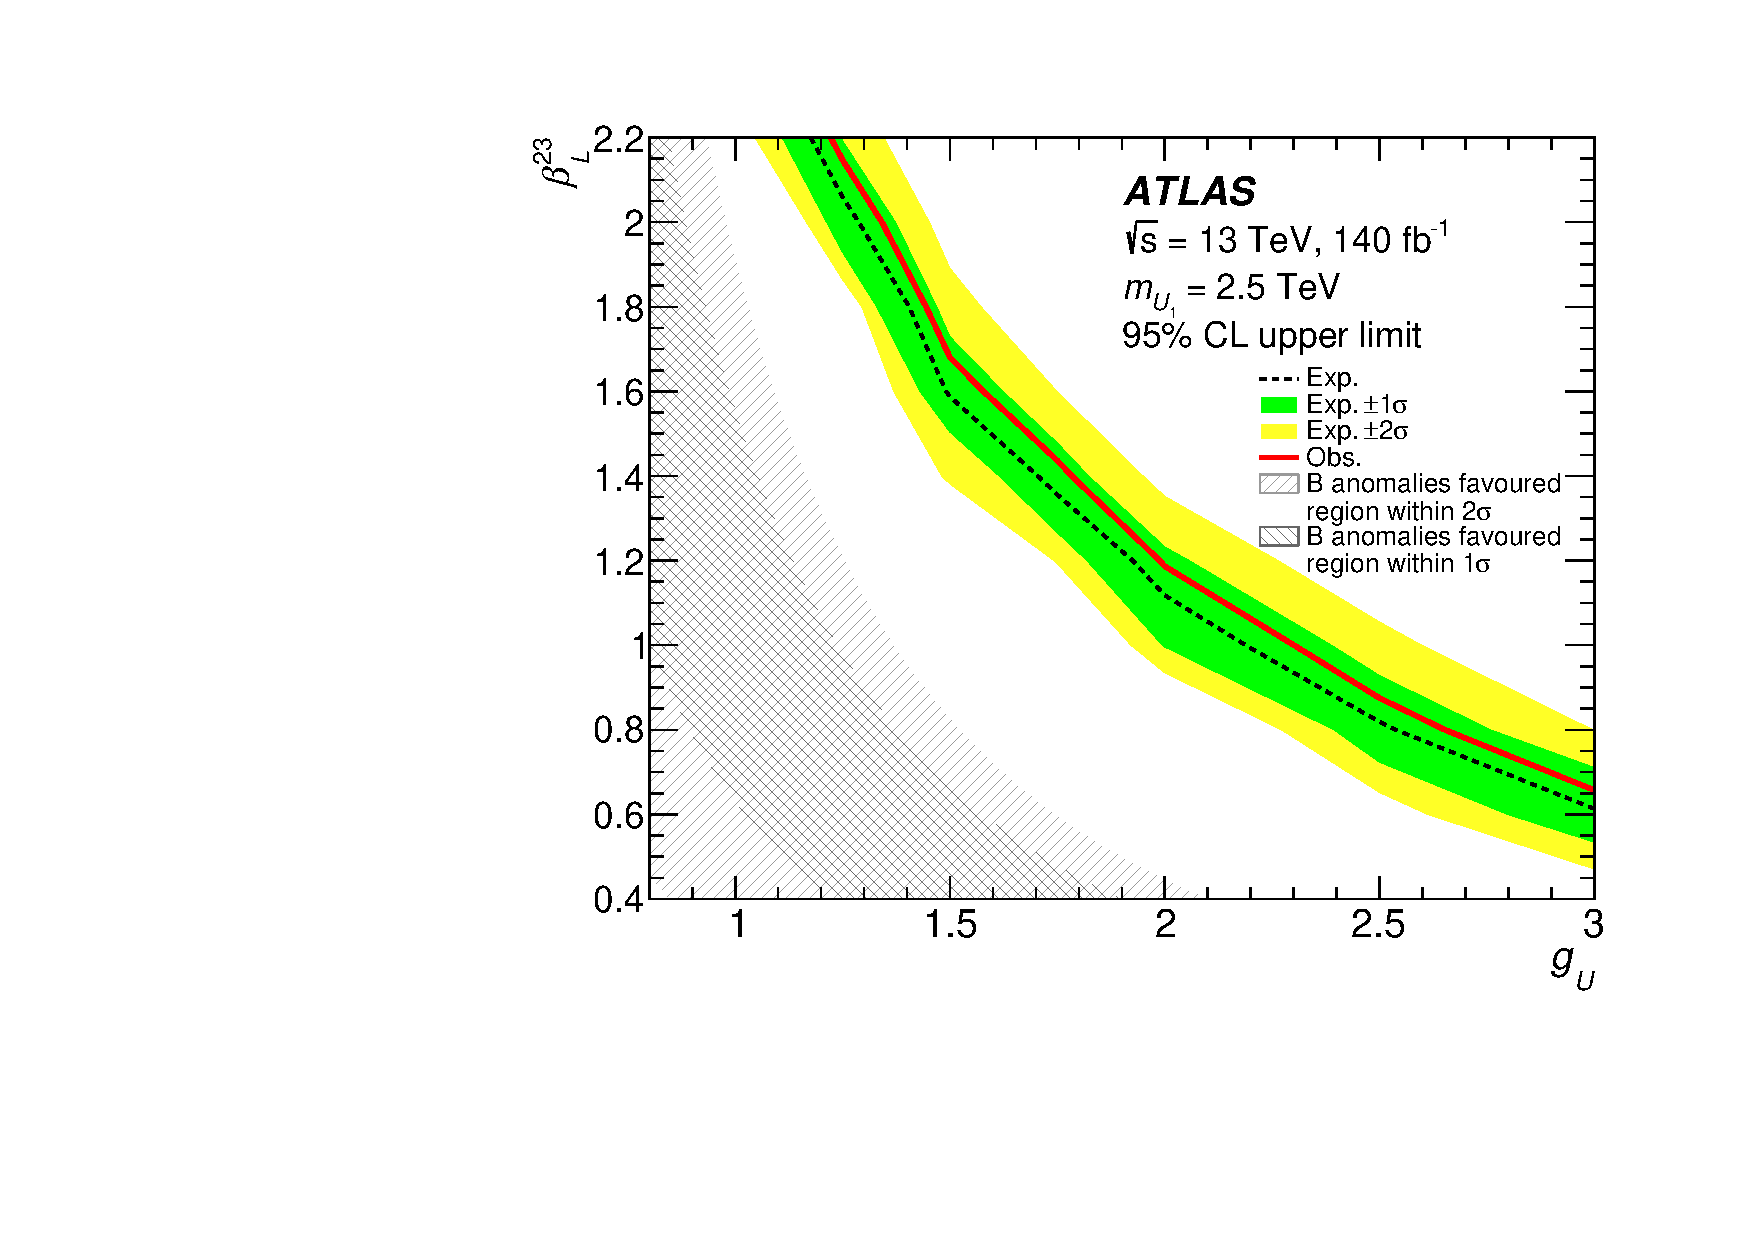
\includegraphics[width=\linewidth]{Figs/CH10/limit_mu2500.pdf}\caption{}\end{subfigure}\hfill
 \begin{subfigure}{0.47\linewidth}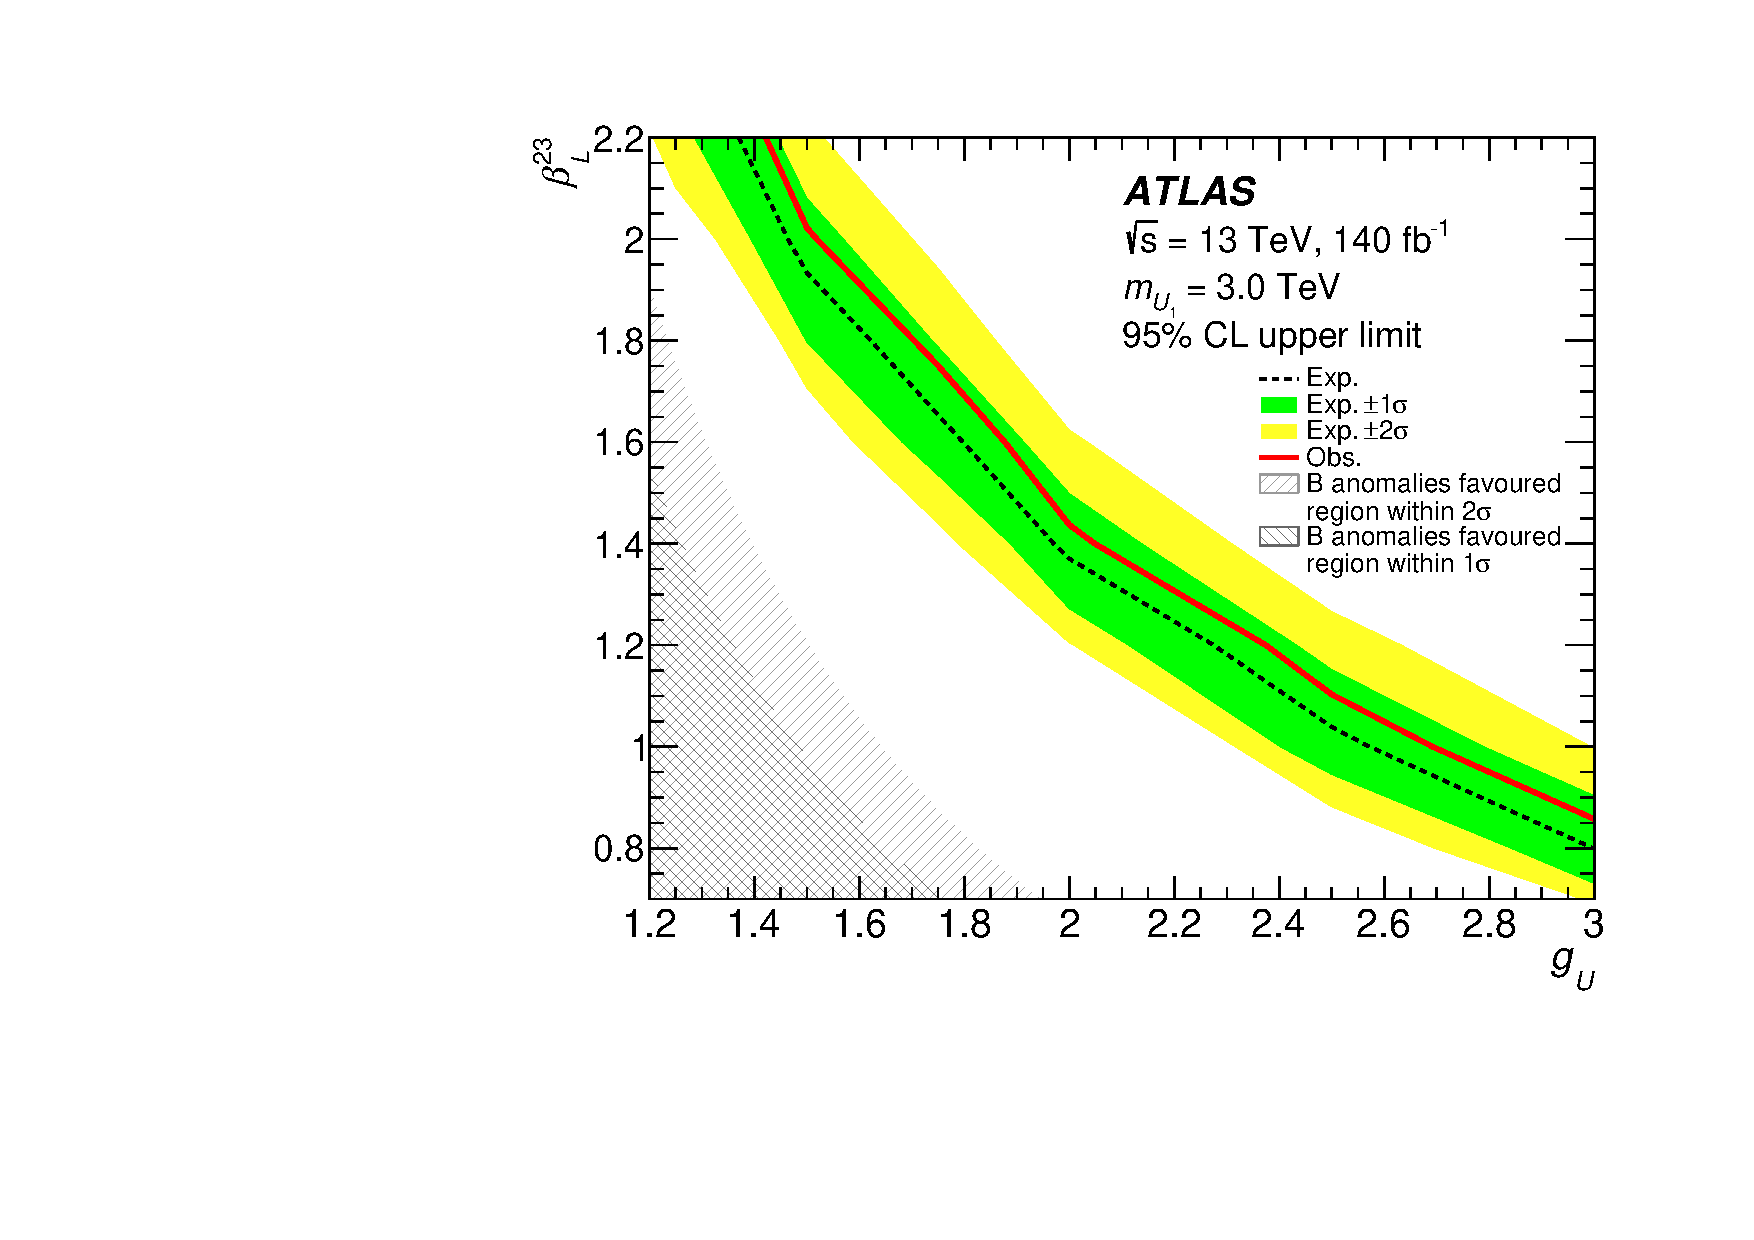
\includegraphics[width=\linewidth]{Figs/CH10/limit_mu3000.pdf}\caption{}\end{subfigure}
 \caption[Exclusions in the two-coupling plane]{Observed (red full line) and expected (black dashed line) 95\% CL upper limits on $\beta_L^{23}$ as a function of $\gU$ at (a) $\MU=1.5~\TeV$, (b) $2.0~\TeV$, (c) $2.5~\TeV$ and (d) $3.0~\TeV$. The shaded regions are favoured by $B$ anomalies at the $1\sigma$ and $2\sigma$ levels, converted from the $C_{LL}^{c}$ limit in Fig.~\ref{fig:cll_clr_low_energy_fit} using Eq.~\eqref{eq:cll_c_approx}.}
 \label{fig:ch10_limits_couplings}
\end{figure}

\clearpage
\subsection{right-handed scenario}
\label{subsec:ch10_rh}

The interpretation for the right-handed scenario uses the signals at $|\beta_R^{33}|=1$ and $\beta_L^{33}=1$ introduced in Section~\ref{subsec:u1_low_energy_fit}.
The signal yields are obtained with the reweighting procedure described in Section~\ref{sec:signal_samples}.

Figure~\ref{fig:ch10_rh_visible_xsec} compares the observed 95\% CL upper limits on the visible cross section for $|\beta_R^{33}|=0$ and 1 at $\gU=1$ and $\beta_L^{23}=0.2$, without considering the interference.
It is defined as:
\begin{align}
 \sigma_{\mathrm{vis}}^{95}=\mu^{95}\sigma A\epsilon,
 \label{eq:ch10_visible_xsec_limit}
\end{align}
where $\sigma$ is the theoretical signal cross section. $A$ and $\epsilon$ are the signal acceptance and selection efficiency, respectively. $\mu^{95}$ is the observed upper limit on $\mu$.

Compared with the purely left-handed scenario, the non-resonant contribution is enhanced more strongly than the resonant contribution in the right-handed scenario.
For non-zero $\beta_R^{33}$, an additional contribution to non-resonant $\tau\nu$ production is generated through the $b_R\tau_R$ coupling, while the $c_L\nu_\tau$ coupling is left unchanged.
For resonant production involve the $b\tau$ coupling, the branching fraction is increased by the additional right-handed coupling, but its enhancement is partly offset by the increase in the total LQ width. Therefore the enhancement is smaller than that of the non-resonant contribution.
The visible cross-section limit is therefore lower for $|\beta_R^{33}|=1$ at $\MU=4~\TeV$.

\begin{figure}[htpb]
 \centering
 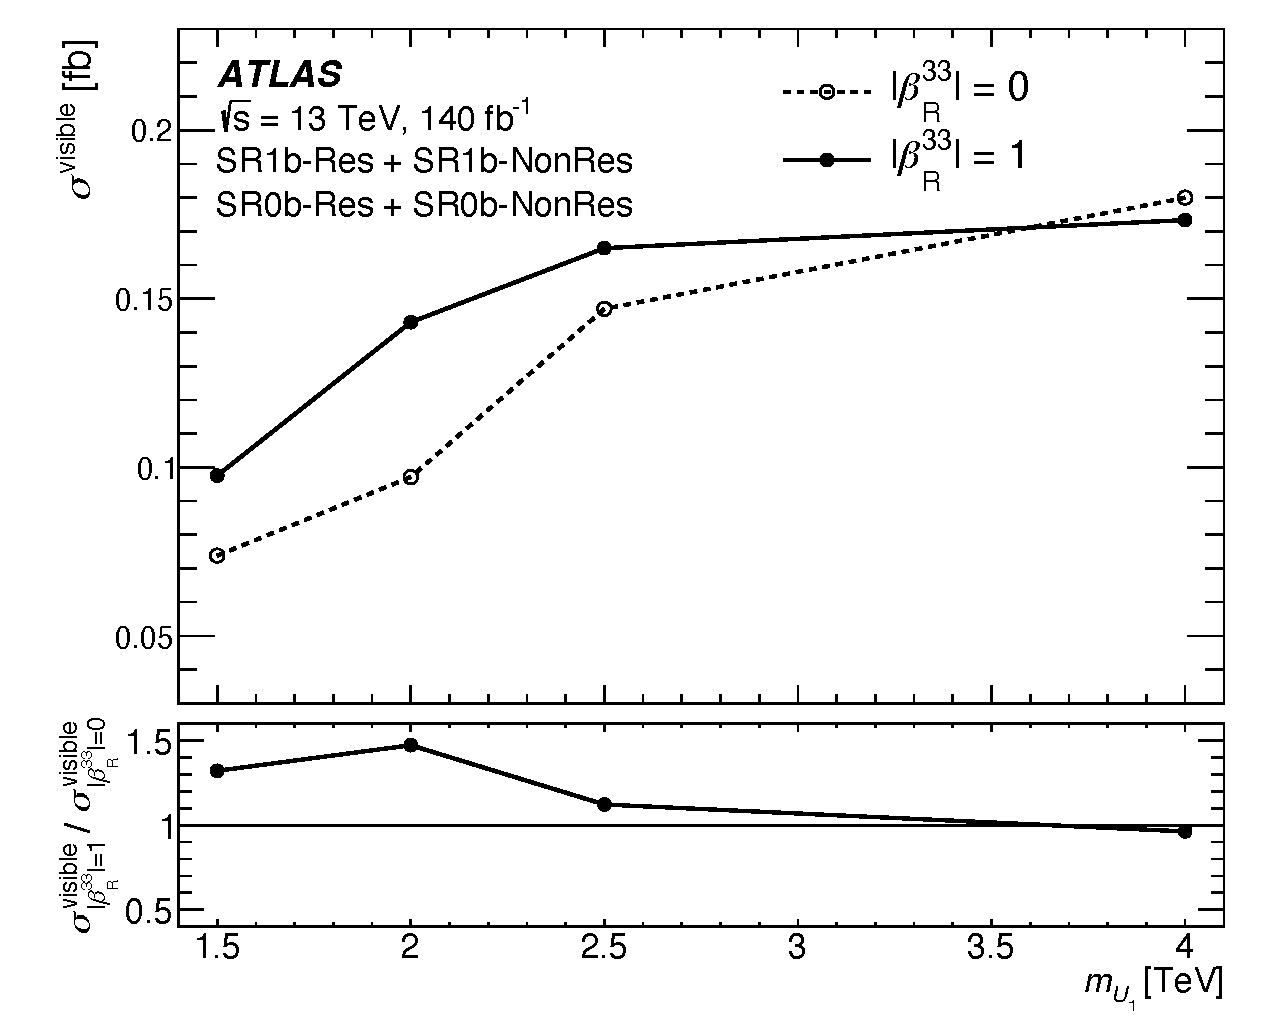
\includegraphics[width=0.7\linewidth]{Figs/CH10/visible_xsec_lh_rh.pdf}
 \caption[Visible cross-section limits for the left- and right-handed scenarios]{The 95\% CL upper limits on the inclusive visible cross section, with $|\beta_R^{33}|=0$ (blank circle) and $|\beta_R^{33}|=1$ (full circle), as a function of $\MU$. The parameters $\gU$ and $\beta_L^{23}$ are fixed at 1 and 0.2, respectively.
 The visible cross section is defined as the cross section calculated with \textsc{MadGraph}, multiplied by the acceptance and selection efficiency.
 All signal regions are combined for simplicity.
 The interference effect with the SM $\tau\nu$ process is not considered.}
 \label{fig:ch10_rh_visible_xsec}
\end{figure}

For the exclusion limit interpretation in the right-handed scenario, the limits are calculated with the asymptotic approximation and without interference, as specified in Section~\ref{subsec:ch10_limit_calculation}.
Figures~\ref{fig:ch10_rh_limits_mass} and~\ref{fig:ch10_rh_limits_couplings} show the 95\% CL exclusion limits.
At $\MU=1.5~\TeV$, the observed (expected) upper limits on $\gU$ are approximately 0.84 (0.80) and 0.53 (0.51) for $\beta_L^{23}=1.0$ and 2.2, respectively.
At $\MU=3.0~\TeV$, the corresponding limits are 1.98 (1.96) and 1.30 (1.28).
A similar dependence on $\gU$ and $\beta_L^{23}$ to that in the left-handed scenario is observed. Note that the hatched regions are recalculated using Eq.~\eqref{eq:cll_c_approx} with $C_{LL}^{c}$ values read from the black solid line of $C_{LR}^{c}=-C_{LL}^{c}$ in Figure~\ref{fig:cll_clr_low_energy_fit}.


\begin{figure}[htpb]
 \centering
 \begin{subfigure}{0.47\linewidth}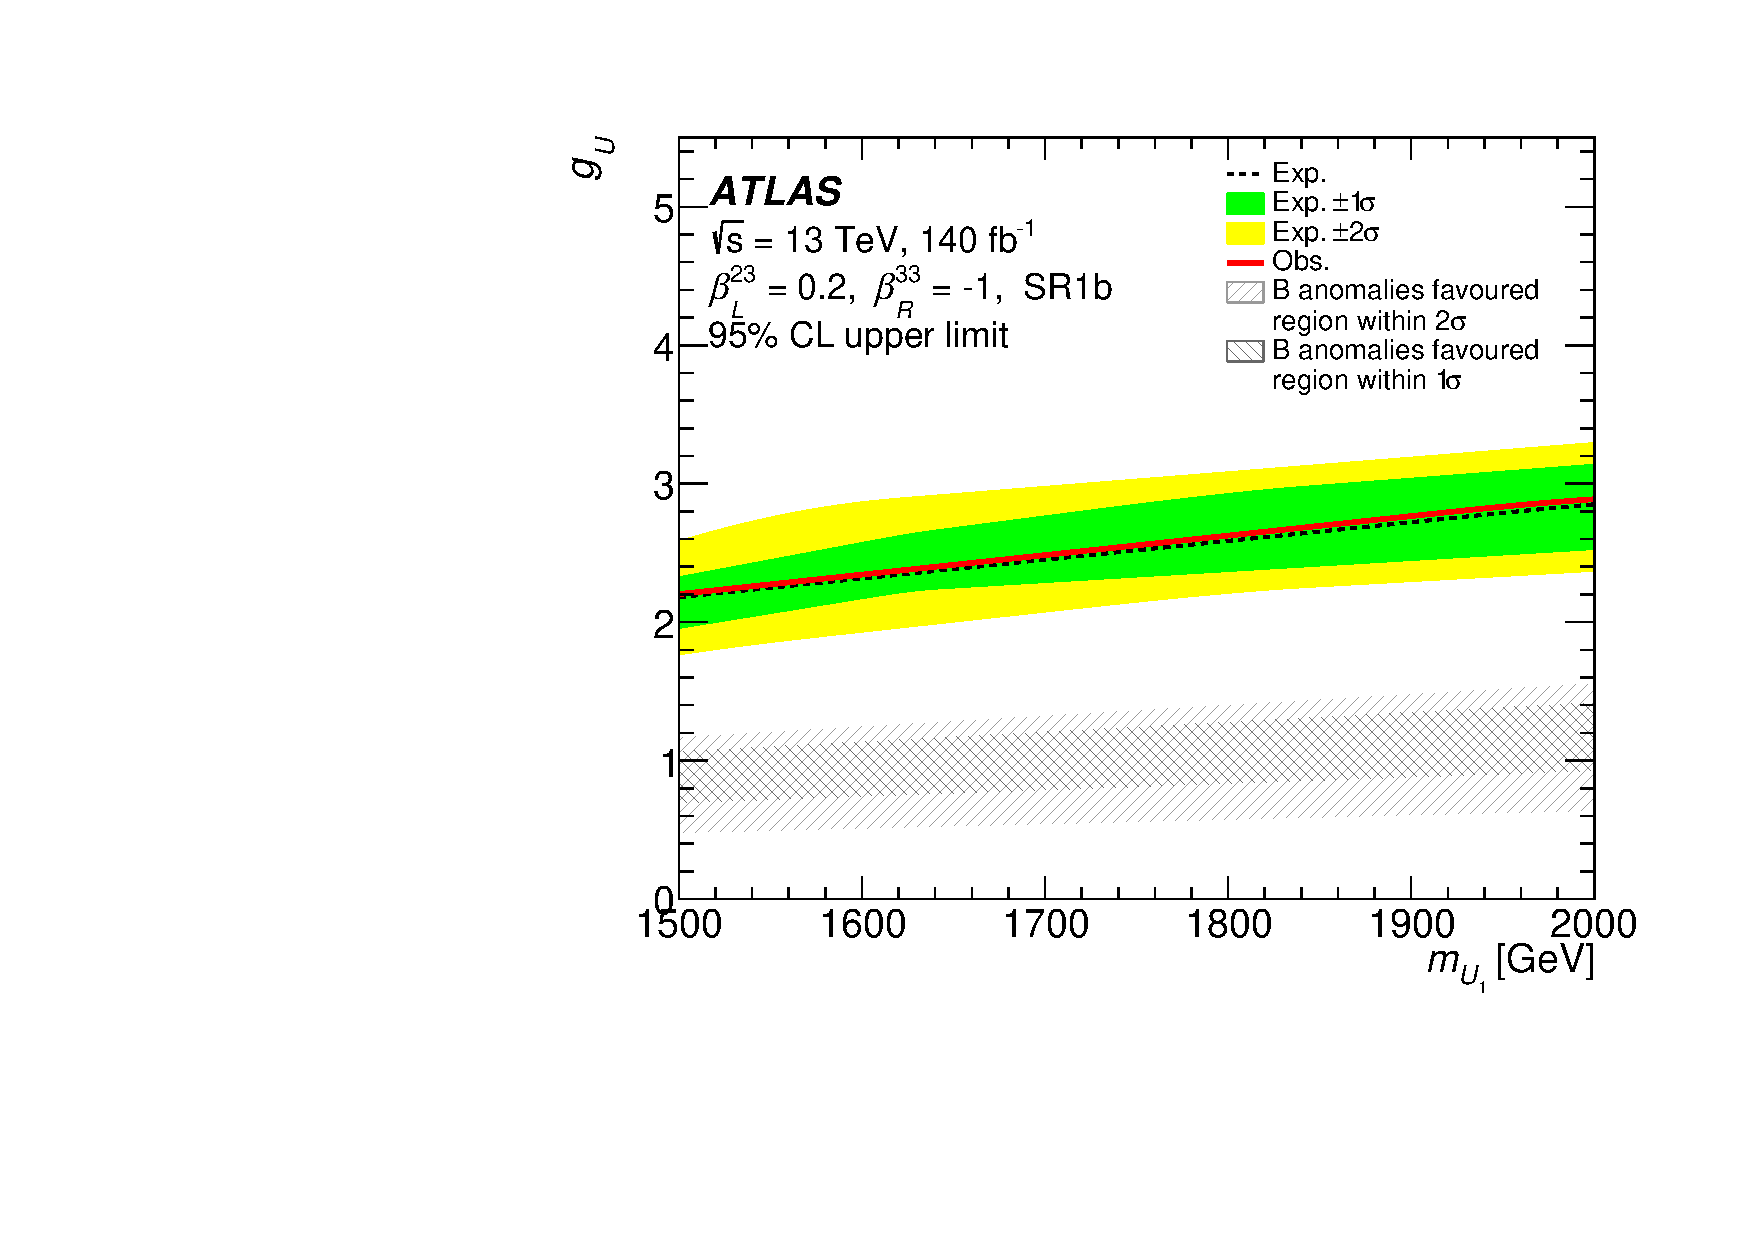
\includegraphics[width=\linewidth]{Figs/CH10/rh_limit_beta0_2.pdf}\caption{}\end{subfigure}\\
 \begin{subfigure}{0.47\linewidth}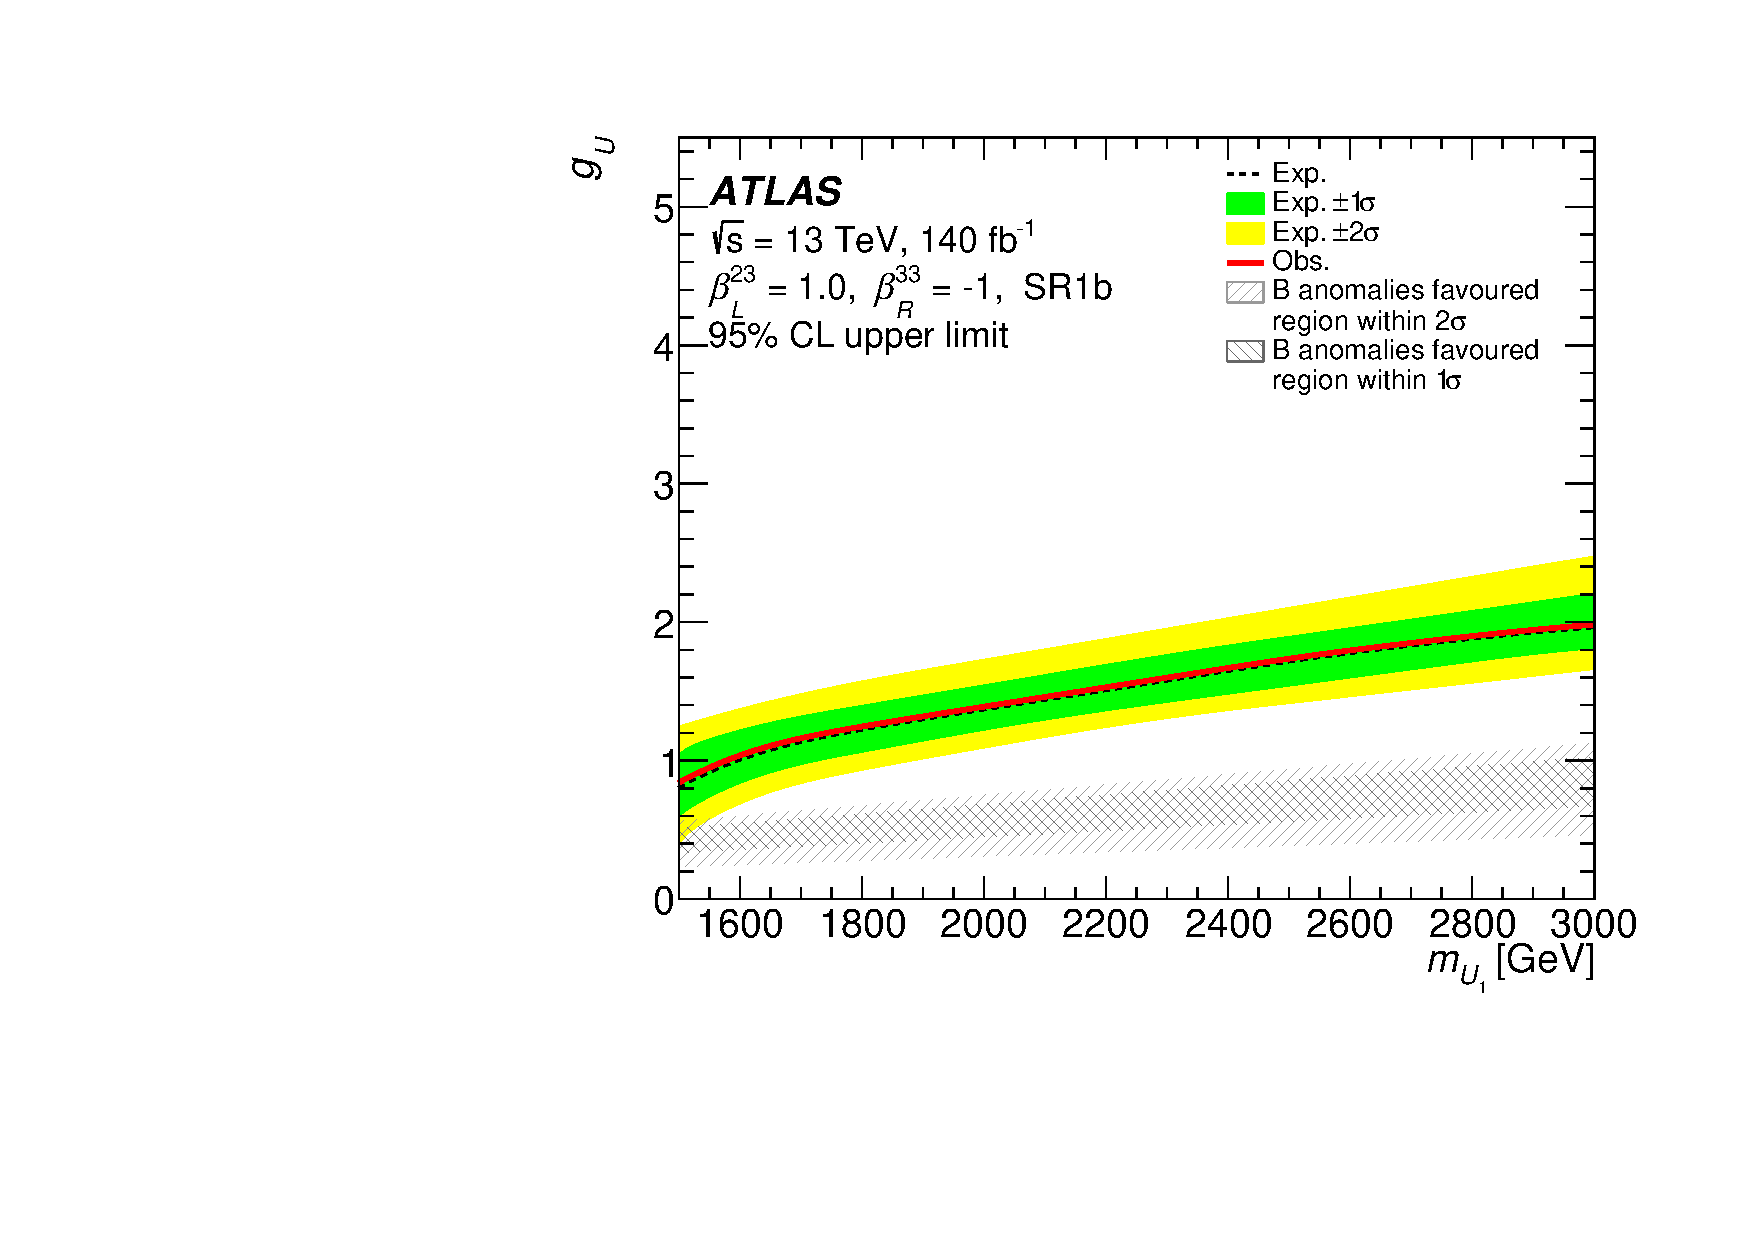
\includegraphics[width=\linewidth]{Figs/CH10/rh_limit_beta1_0.pdf}\caption{}\end{subfigure}\hfill
 \begin{subfigure}{0.47\linewidth}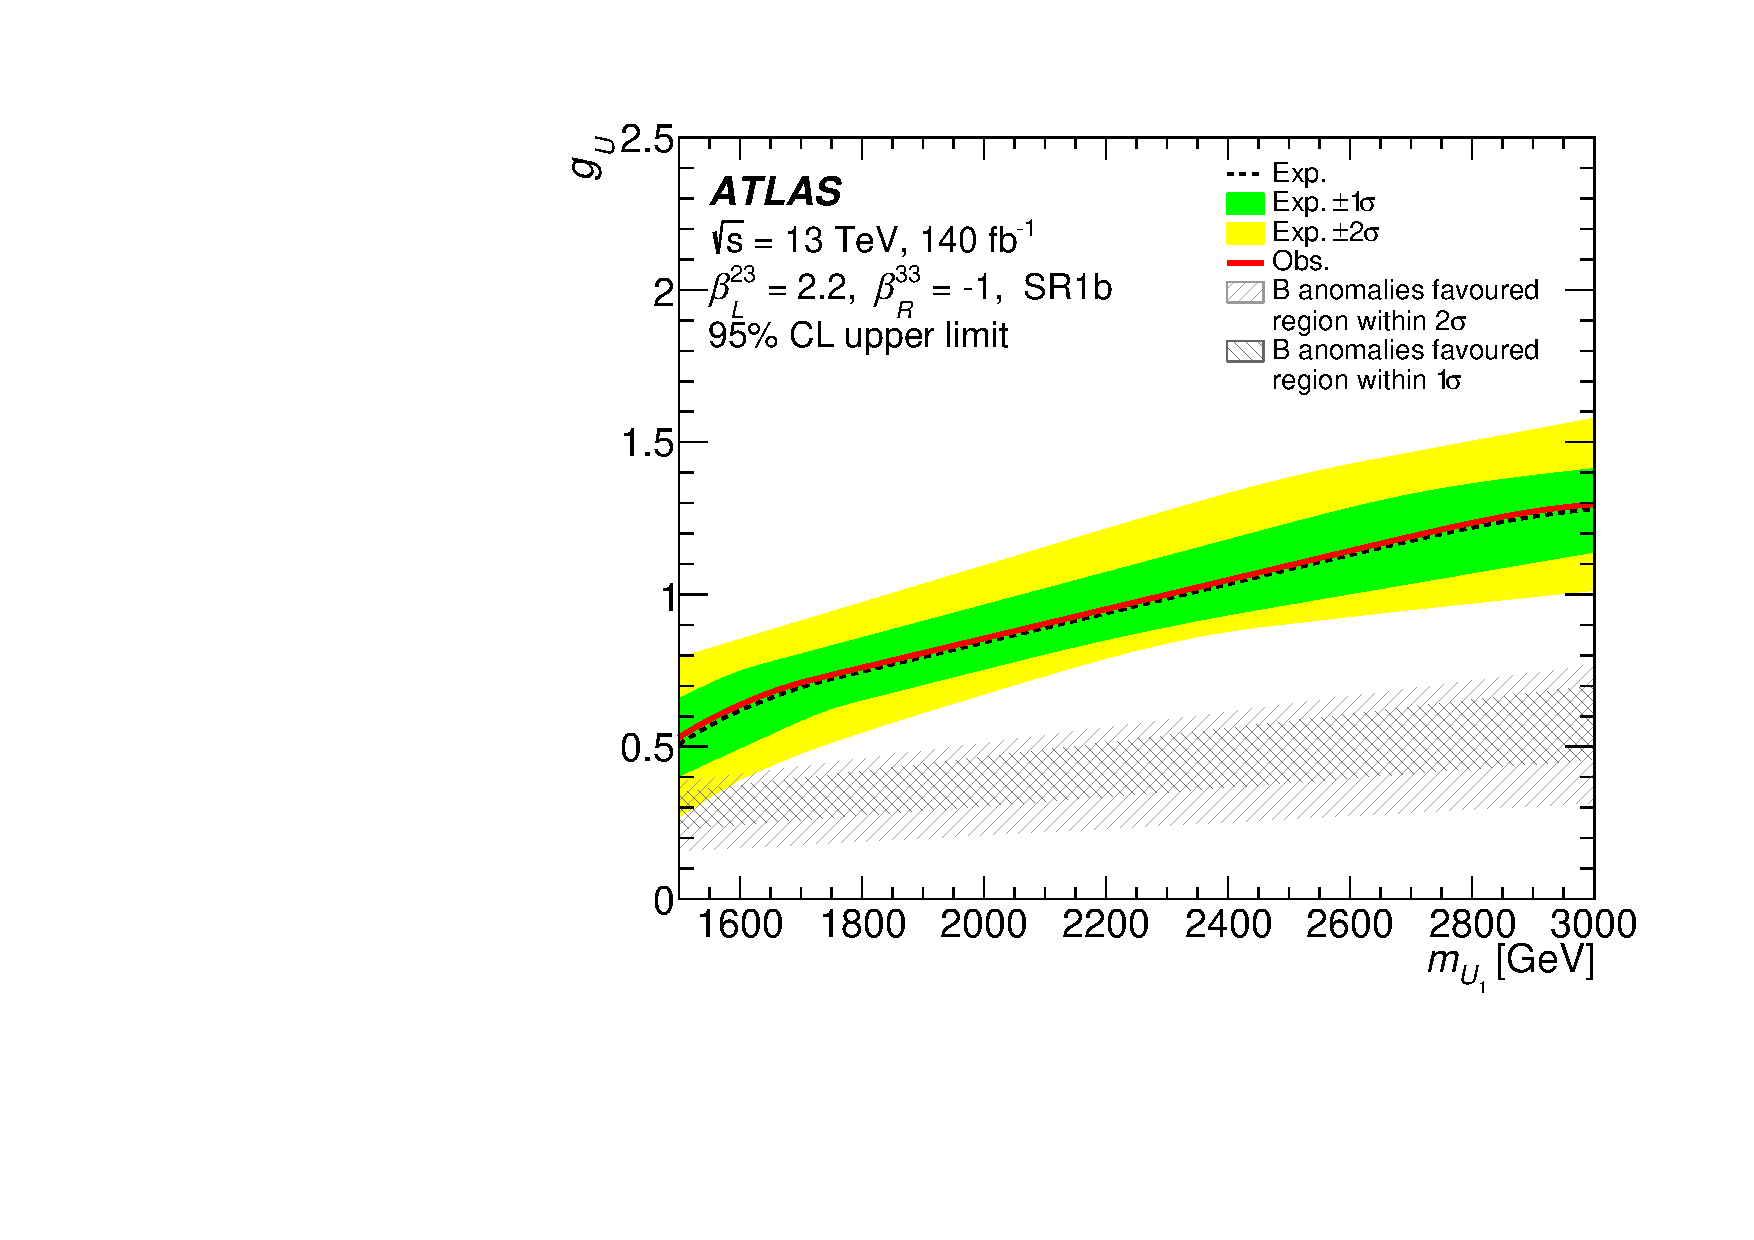
\includegraphics[width=\linewidth]{Figs/CH10/rh_limit_beta2_2.pdf}\caption{}\end{subfigure}
 \caption[Right-handed limits on the coupling as a function of the leptoquark mass]{Observed (red full line) and expected (black dotted line) 95\% CL upper limits on $\gU$ as a function of $\MU$ for $\beta_R^{33}=-1$, at (a) $\beta_L^{23}=0.2$, (b) 1.0 and (c) 2.2. The hatched regions are recalculated using Eq.~\eqref{eq:cll_c_approx} with $C_{LL}^{c}$ values read from the black solid line of $C_{LR}^{c}=-C_{LL}^{c}$ in Figure~\ref{fig:cll_clr_low_energy_fit}.}
 \label{fig:ch10_rh_limits_mass}
\end{figure}

\begin{figure}[htpb]
 \centering
 \begin{subfigure}{0.47\linewidth}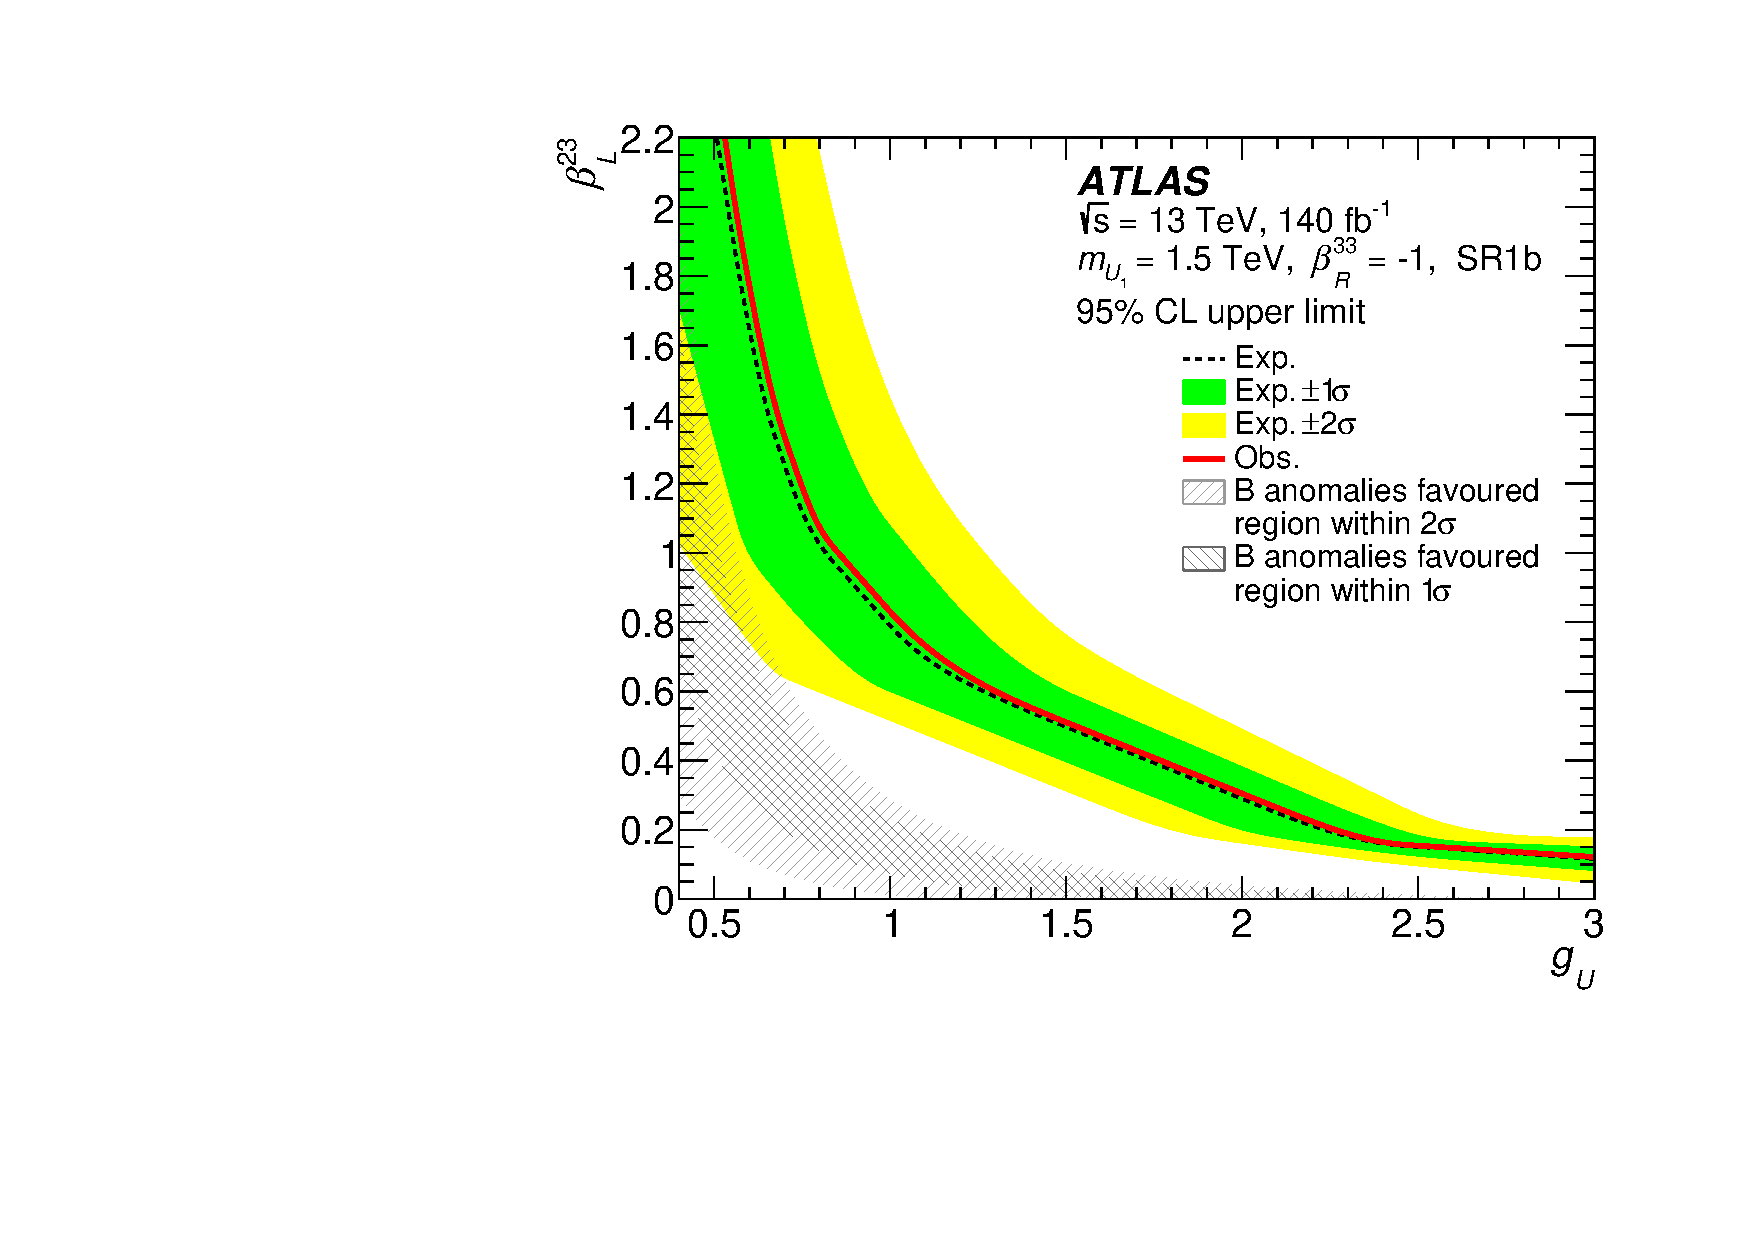
\includegraphics[width=\linewidth]{Figs/CH10/rh_limit_mu1500.pdf}\caption{}\end{subfigure}\hfill
 \begin{subfigure}{0.47\linewidth}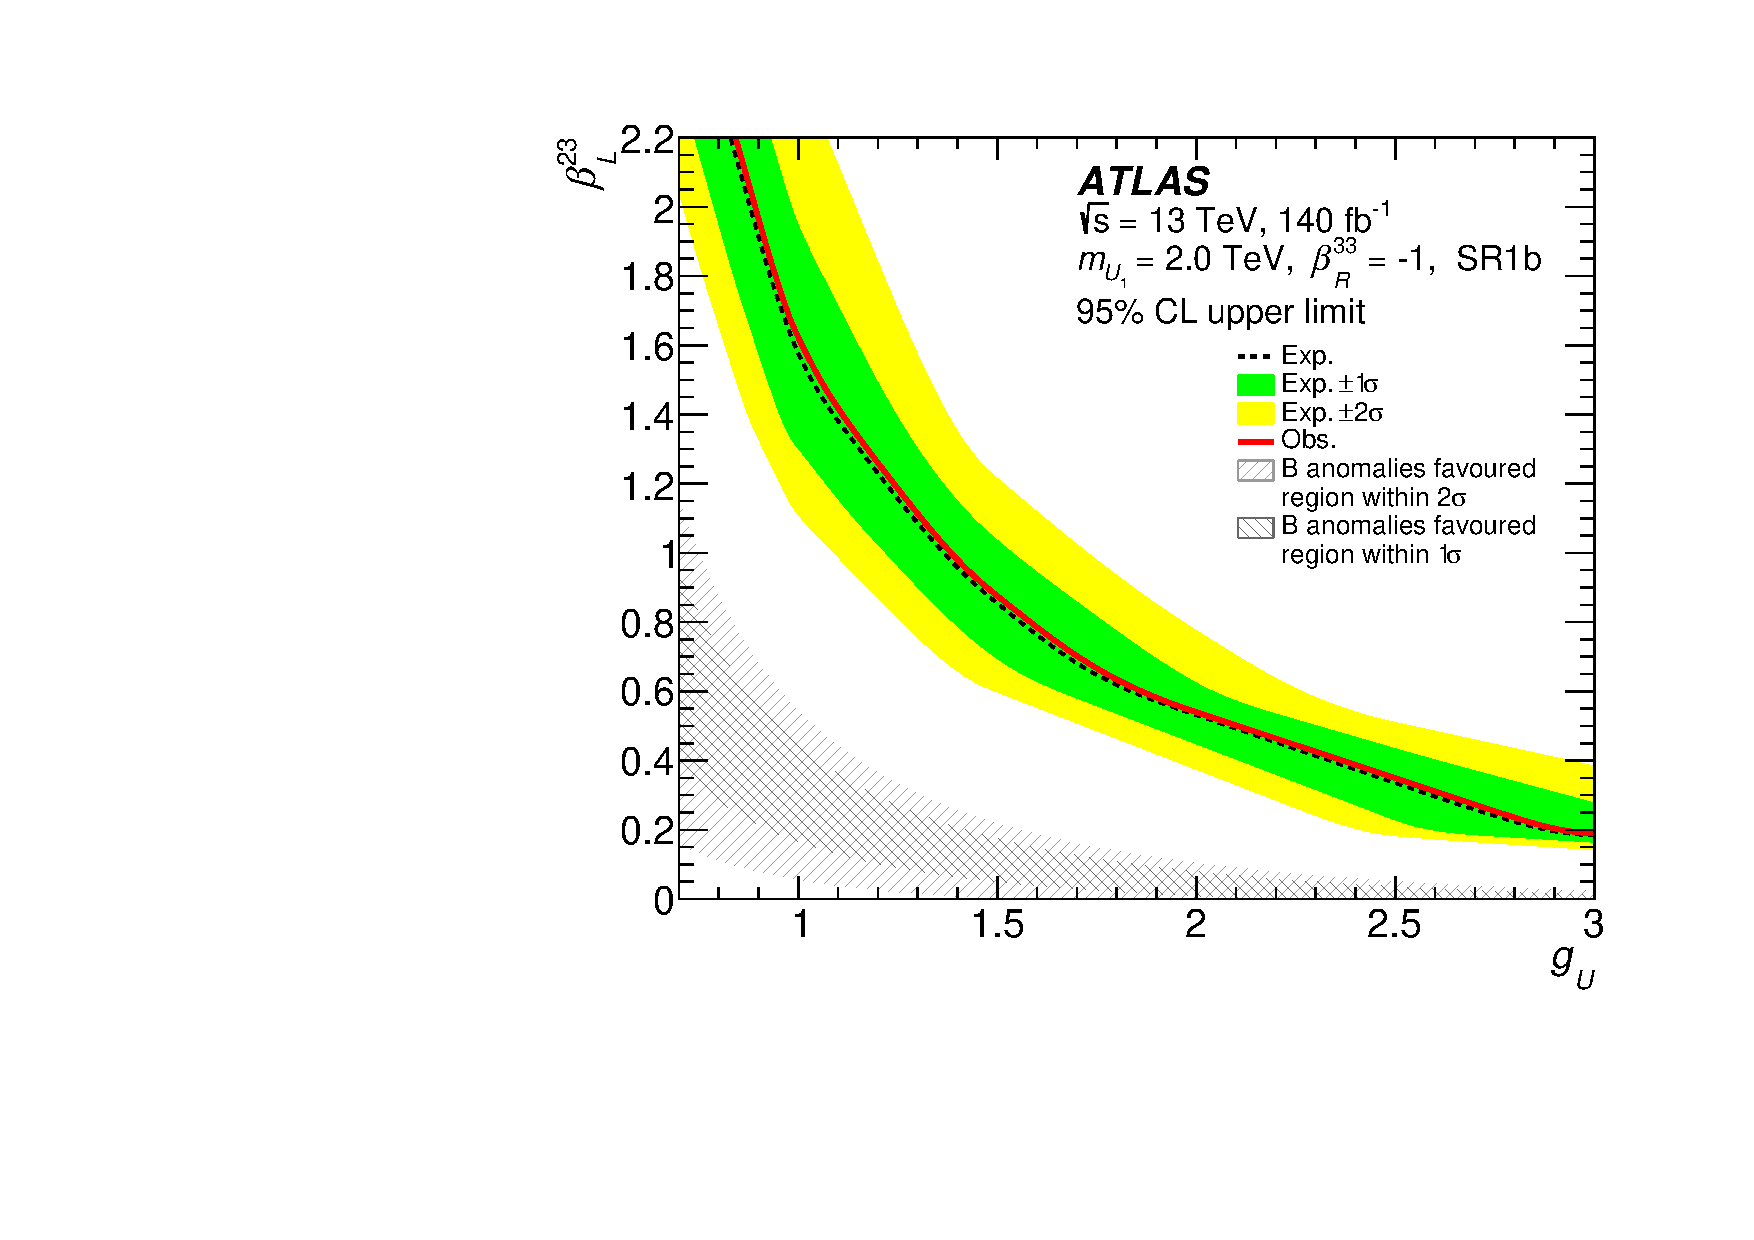
\includegraphics[width=\linewidth]{Figs/CH10/rh_limit_mu2000.pdf}\caption{}\end{subfigure}\\
 \begin{subfigure}{0.47\linewidth}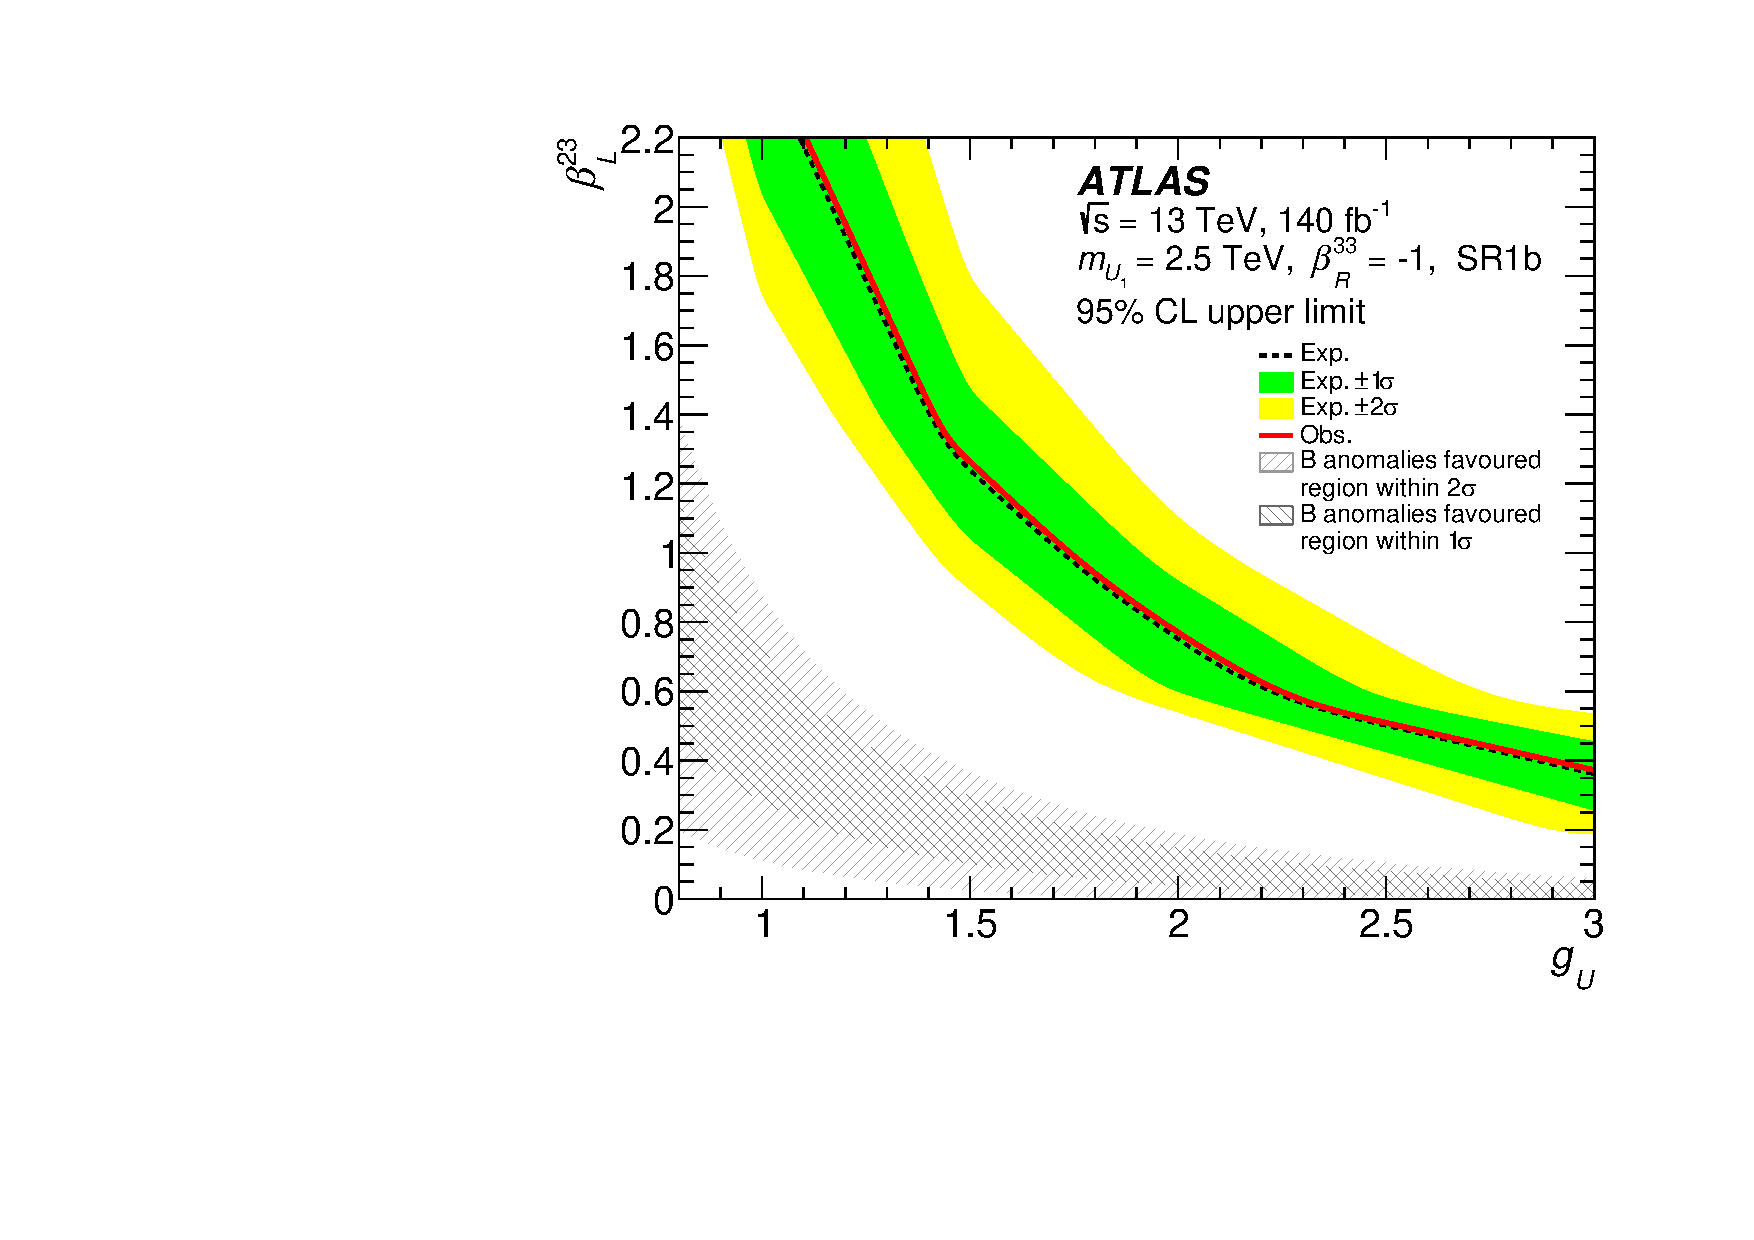
\includegraphics[width=\linewidth]{Figs/CH10/rh_limit_mu2500.pdf}\caption{}\end{subfigure}\hfill
 \begin{subfigure}{0.47\linewidth}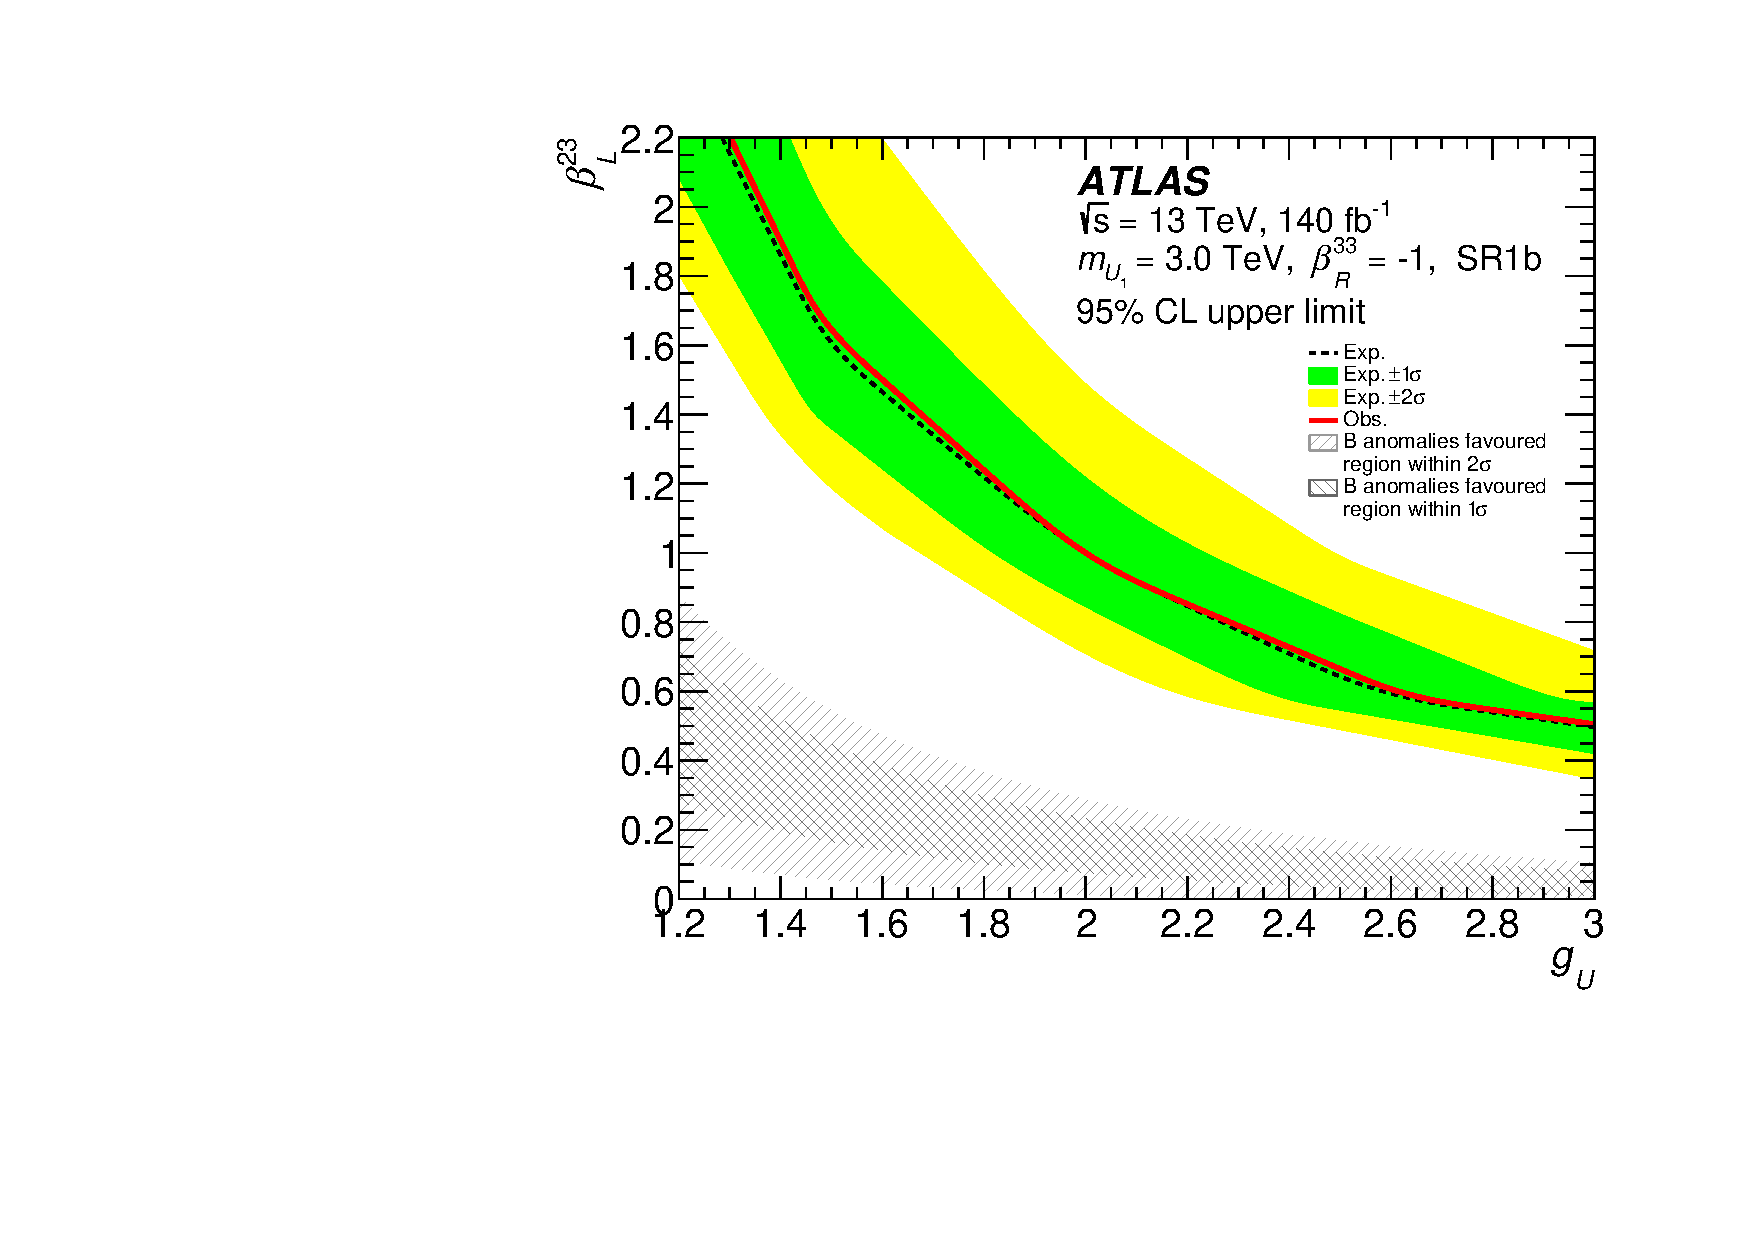
\includegraphics[width=\linewidth]{Figs/CH10/rh_limit_mu3000.pdf}\caption{}\end{subfigure}
 \caption[Right-handed exclusions in the two-coupling plane]{Observed (red full line) and expected (black dotted line) 95\% CL upper limits on $\beta_L^{23}$ as a function of $\gU$ for $\beta_R^{33}=-1$ at (a) $\MU=1.5~\TeV$, (b) $2.0~\TeV$, (c) $2.5~\TeV$ and (d) $3.0~\TeV$. The hatched regions are recalculated using Eq.~\eqref{eq:cll_c_approx} with $C_{LL}^{c}$ values read from the black solid line of $C_{LR}^{c}=-C_{LL}^{c}$ in Figure~\ref{fig:cll_clr_low_energy_fit}.}
 \label{fig:ch10_rh_limits_couplings}
\end{figure}

\clearpage
\section{Future improvements}
\label{sec:ch10_future}

The coupling limits are expected to improve only modestly with the larger datasets from Run~3 and the HL-LHC.
An illustrative projection study compares expected limits at $140~\ifb$ with those at $450~\ifb$ and $3000~\ifb$ using Asimov datasets at $\sqrt{s}=13~\TeV$ with the same selections.
For $\MU=3.0~\TeV$ and $\beta_L^{23}=1.4$, the expected 95\% CL upper limit on $\gU$ improved by approximately $5\%$ and $10\%$ at $450~\ifb$ and $3000~\ifb$, respectively, compared with $140~\ifb$.
This limited gain is expected due to the approximate $\gU^4$ dependence of the non-resonant pure-BSM contribution at fixed $\MU$ and $\beta_L^{23}$.
Further improvements are therefore expected from reoptimising the selections in addition to increasing the integrated luminosity.

The right-handed interpretation should be extended with interference included in the limit calculation.
The existing limits neglect this contribution, while the study at $\MU=1.5~\TeV$ indicates sizeable interference in $\bVetoSR$.
Additional interference samples covering masses and couplings in the full range of interest are therefore needed.

The sensitivity could be improved through a dedicated optimisation of $\bVetoSR$, whose selections were inherited from the $\bTagSR$.
A preliminary study with selected leading systematic uncertainties found improved sensitivity with $\met>600~\GeV$ in $\bVetoSR$-\Res.
The higher threshold favours events containing an energetic neutrino from an on-shell $U_1\to c\nu_\tau$ decay, while suppressing the softer $\wjets$ background.
The magnitude of the interference compared with the pure-BSM yield is also reduced in such phase space.
This optimisation was not applied in this thesis, and its potential gain should be reassessed in a future analysis.
